\documentclass[10pt, a4paper,english,spanish,hidelinks]{article}
\usepackage{amsmath}
\usepackage{amsfonts}
\usepackage{amssymb}
\usepackage{caratula}
\usepackage[spanish, activeacute]{babel}
\usepackage[usenames,dvipsnames]{color}
\usepackage[width=15.5cm, left=3cm, top=2.5cm, height= 24.5cm]{geometry}
\usepackage{graphicx}
\usepackage[utf8]{inputenc}
\usepackage{listings}
\usepackage{multicol}
%\usepackage{subfig}
\usepackage{float}
\usepackage{color,hyperref}
\usepackage{listings}
\usepackage{caption}
\usepackage{subcaption}

\usepackage{listings}
\usepackage{babel}
\usepackage{url}
\usepackage{lscape}
\parindent = 15 pt
\parskip = 11 pt

\usepackage{fancyhdr}
\usepackage{hyperref}
\usepackage{amsmath}
\usepackage{amsfonts}
\usepackage{amssymb}
\usepackage[utf8]{inputenc}
\usepackage{graphicx}
\usepackage{caption}
\usepackage{color}
%\usepackage{appendix}
\usepackage{fancyhdr}
\usepackage{graphicx}


\materia{Teoría de las Comunicaciones}

\titulo{Trabajo Práctico 2}
\fecha{14 de Julio de 2015}
\integrante{Gauder, Maria Lara}{027/10}{marialaraa@gmail.com}
\integrante{Kovacs, Ignacio Javier}{627/10}{ignacio.k91@gmail.com}
\integrante{Puerta, Armando Ezequiel}{812/09}{eze19.2009@gmail.com}
\integrante{Reartes, Marisol}{422/10}{mreartes5@gmail.com}

\begin{document}
\pagestyle{myheadings}
\maketitle
\markboth{Teoría de las Comunicaciones}{Rutas en Internet}

\thispagestyle{empty}
\tableofcontents
\newpage

\section{Introducción}

A lo largo de este trabajo práctico se experimentará con técnicas
y herramientas utilizadas a nivel de red. Particularmente, se analizará
la herramienta \textit{traceroute} junto con los protocolos involucrados de esa capa. 

Para realizar los experimentos se eligieron cuatro universidades distintas: la Universidad Humboldt de Berlín, la Universidad de Moscú,
la Universidad de Tokio y la Universidad de Boston.

Se desarrollara y aplicará una herramienta que permitirá analizar el comportamiento de un paquete en la red. 

El trabajo práctico se divide en tres partes. La primera hace referencia a la herramienta de traceroute y la realización de cálculos a partir de los datos obtenidos. Luego, se plasmarán los mismos en diversos gráficos y diagramas para poder definir ciertos escenarios esperados. Por último, se aplicará otra herramienta para poder contrastar con la realidad cierto comportamiento teórico. 

\newpage
\section{Caracterizando rutas}

A partir de la tool implementada, que permite realizar un \textbf{traceroute}, se pueden obtener los RTT entre cada salto de hops para una ruta a una IP determinada. De esta manera, se plantea en primer lugar 4 universidades diferentes, que serán utilizadas para poder llevar a cabo el análisis necesario utilizando la herramienta.

\begin{itemize}
 \item {\bf Universidad Humboldt de Berlín}

	{\bf Distancia}: 11910 km

	{\bf IP}: 141.20.5.188 (\url{www.hu-berlin.de}{})

 \item {\bf Universidad de Moscú}

	{\bf Distancia}: 13484 km

	{\bf IP}: 188.44.33.1 (\url{www.msu.ru}{})

 \item {\bf Universidad de Boston}

	{\bf Distancia}: 8680 km

	{\bf IP}: 54.230.225.44 (\url{www.bu.edu}{})

 \item {\bf Universidad de Tokio}

	{\bf Distancia}: 18360 km

	{\bf IP}: 210.152.135.178 (\url{www.u-tokyo.ac.jp}{})

\end{itemize}

Las distancias descriptas corresponden a la distancia lineal que hay entre la universidad y un punto en común en Buenos Aires. La misma se obtuvo utilizando una opción dada por Google Maps \footnote{\url{maps.google.com}{}}. Ese dato se podrá utilizar para poder obtener el RTT teórico y aproximado de un paquete para cada una de las universidad a analizar.

Asumiendo que los enlaces son siempre de fibra óptica, y que el velocidad de propagación de las señales es de $2 \times 10^{5}$ km/s podemos estimar el RTT de la siguiente manera:

\begin{itemize}
 \item Universidad Humboldt de Berlín:
\begin{equation}
 	RTT = 2 \times T_{prop} = 2 \times (Dist / V_{prop}) = 2 \times (11910 \text{ km} / 2\times10^5 \text{ km/s}) = 119.1  \text{ ms}
\end{equation}

 \item Universidad de Moscú:
 \begin{equation}
 	RTT = 2 \times T_{prop} = 2 \times (Dist / V_{prop}) = 2 \times (13484 \text{ km} / 2\times10^5 \text{ km/s}) = 134.84 \text{ ms}
 \end{equation}

 \item Universidad de Boston:
 \begin{equation}
 	RTT = 2 \times T_{prop} = 2 \times (Dist / V_{prop}) = 2 \times (8680 \text{ km} / 2\times10^5 \text{ km/s}) = 86.8 \text{ ms}
 \end{equation}

 \item Universidad de Tokio:
 \begin{equation}
 	RTT = 2 \times T_{prop} = 2 \times (Dist / V_{prop}) = 2 \times (18360  \text{ km} / 2\times10^5 \text{ km/s}) = 183.6 \text{ ms}
 \end{equation}

\end{itemize}

El valor obtenido representa un cota inferior muy burda del tiempo de comunicación entre Buenos Aires y las universidades seleccionadas. Esto se debe a que no contempla los obstáculos que se presentan desde que un paquete sale del hop inicial y llega a destino. Hay ciertas situaciones que fomentan un aumento importante del tiempo de RTT del mensaje. Se presenta a continuación, las diferencias entre el RTT teórico y el obtenido utilizando una herramienta brindada por el sistema operativo \footnote{\url{http://ping.eu}{}}.

\centerline{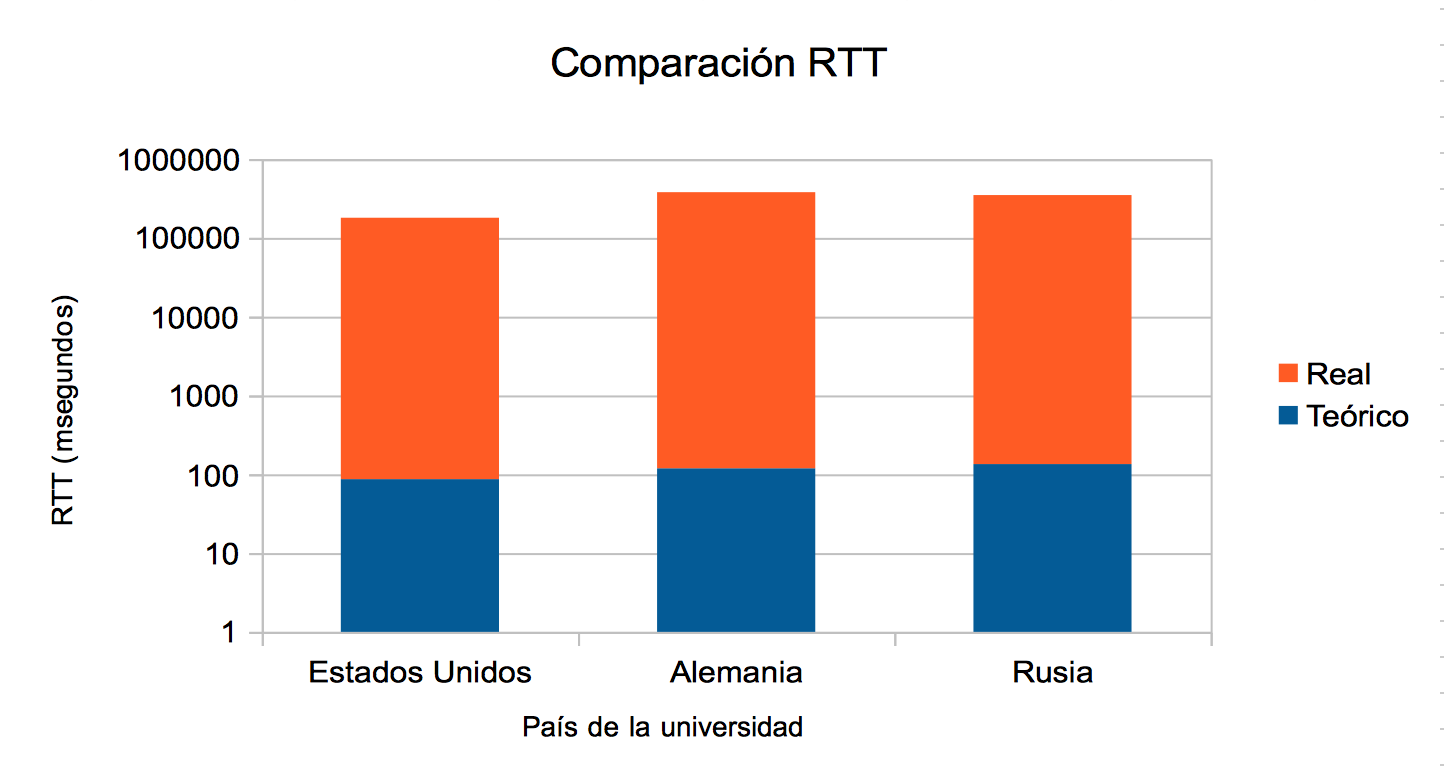
\includegraphics[width=0.8\textwidth]{imagenes/1ra_parte/1Parte-comparacionRTT}}

Se muestran los resultado utilizando escala logarítmica para poder observarlos de manera clara. A lo largo del trabajo práctico se podrán ir observando las situaciones que demuestan el porque el RTT teórico puede valer tanto menos que el de la realidad.

Por otro lado, se decide comparar la herramienta desarrollada utilizando Scapy, contra el traceroute brindado por el sistema operativo. Ambos traceroutes envían una cierta cantidad de paquetes a cada host intermedio que se tiene para llegar al de destino. En el caso de la herramienta desarrollada, esto se logra determinando el valor máximo de TTL que tiene el paquete. Dicho valor representa la cantidad máxima de saltos que puede tener el mensaje enviado. Además, al recibirse la respuesta por parte del hop al que un paquete llega con TTL igual a cero, se mide el tiempo que toma en milisegundos. Este tiempo de ida y vuelta de un paquete se denomina RTT. En el caso de nuestras herramienta desarrollada, se envía mil paquetes con un mismo valor de TTL máximo, y luego se obtiene el RTT aproximado, promediando el de todos. 

A continuación, se presentan los RTT obtenidos para cada hop intermedio utilizando ambas herramientas. 

\centerline{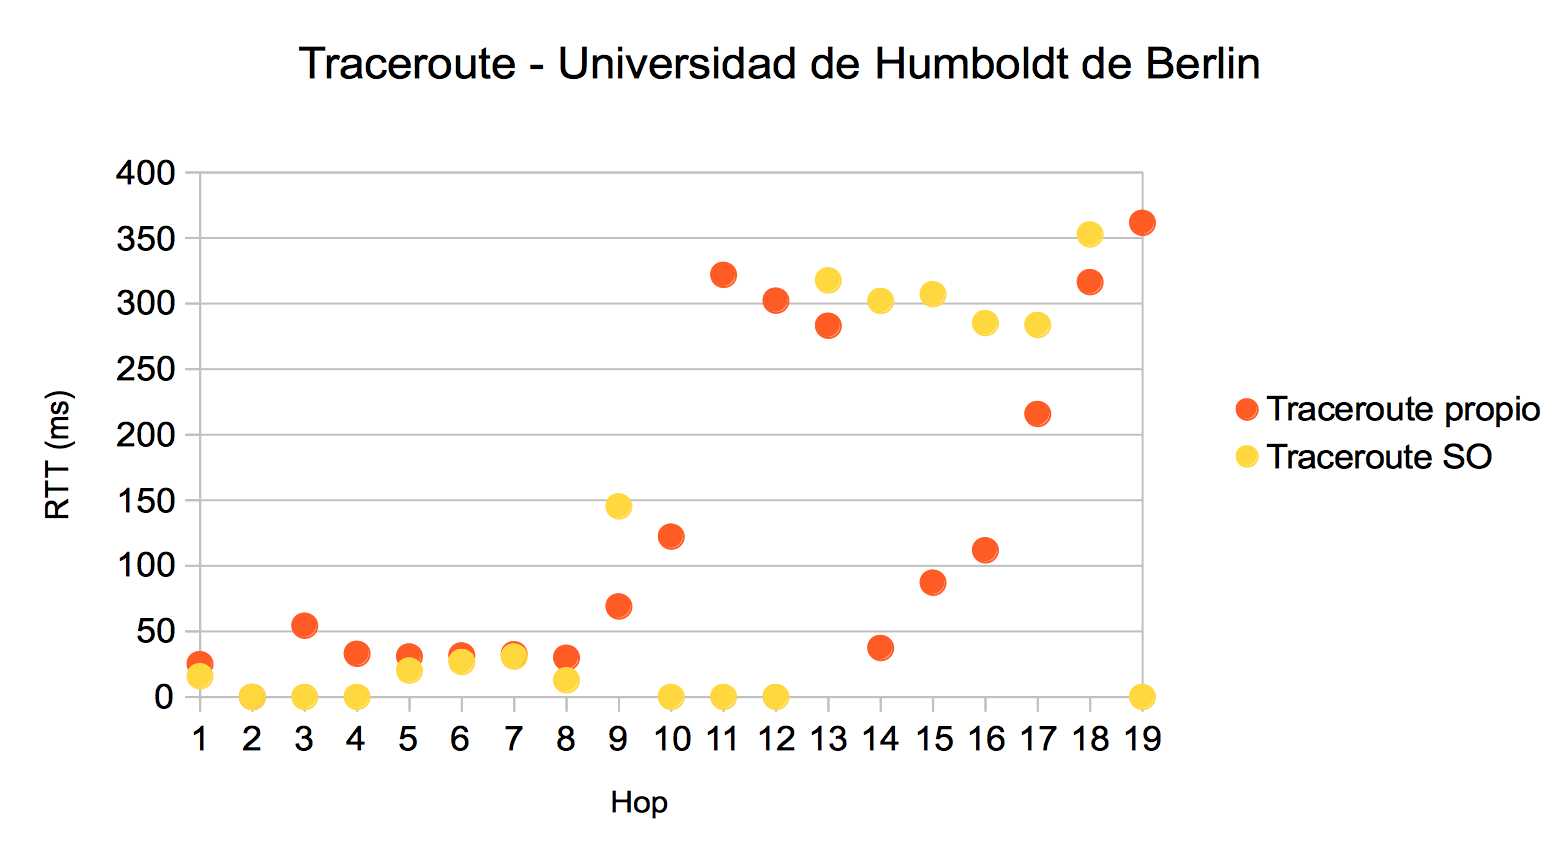
\includegraphics[width=1\textwidth]{imagenes/1ra_parte/Alemania_1ergrafico.png}}

\centerline{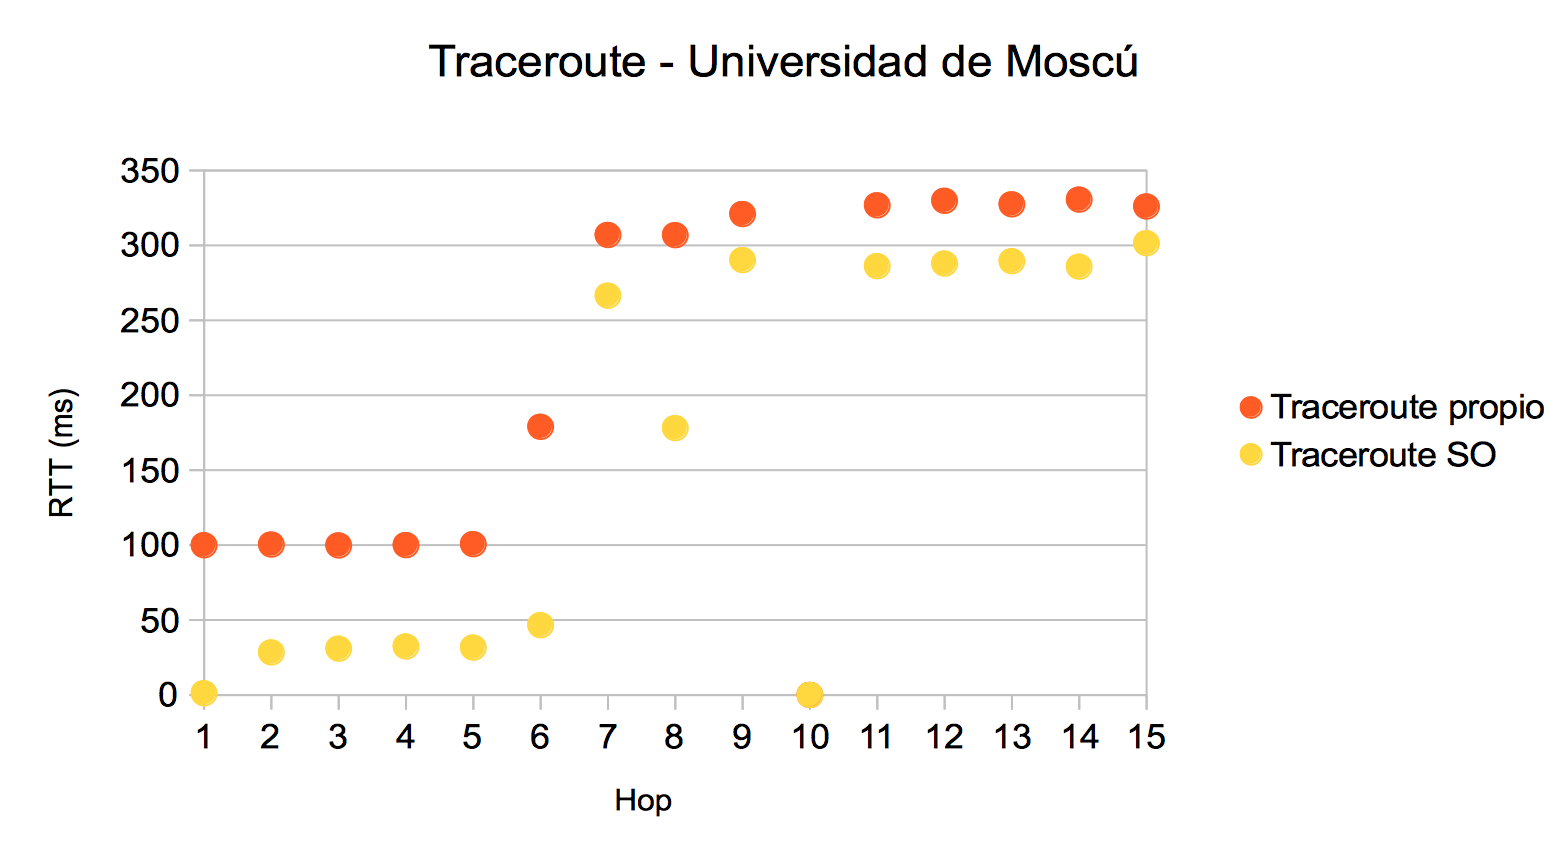
\includegraphics[width=1\textwidth]{imagenes/1ra_parte/Rusia_1ergrafico.png}}

Se observa en este escenario, que las mediciones realizadas por el traceroute desarrollado presenta mediciones más altas, pero probablemente sean más certeras. 

\centerline{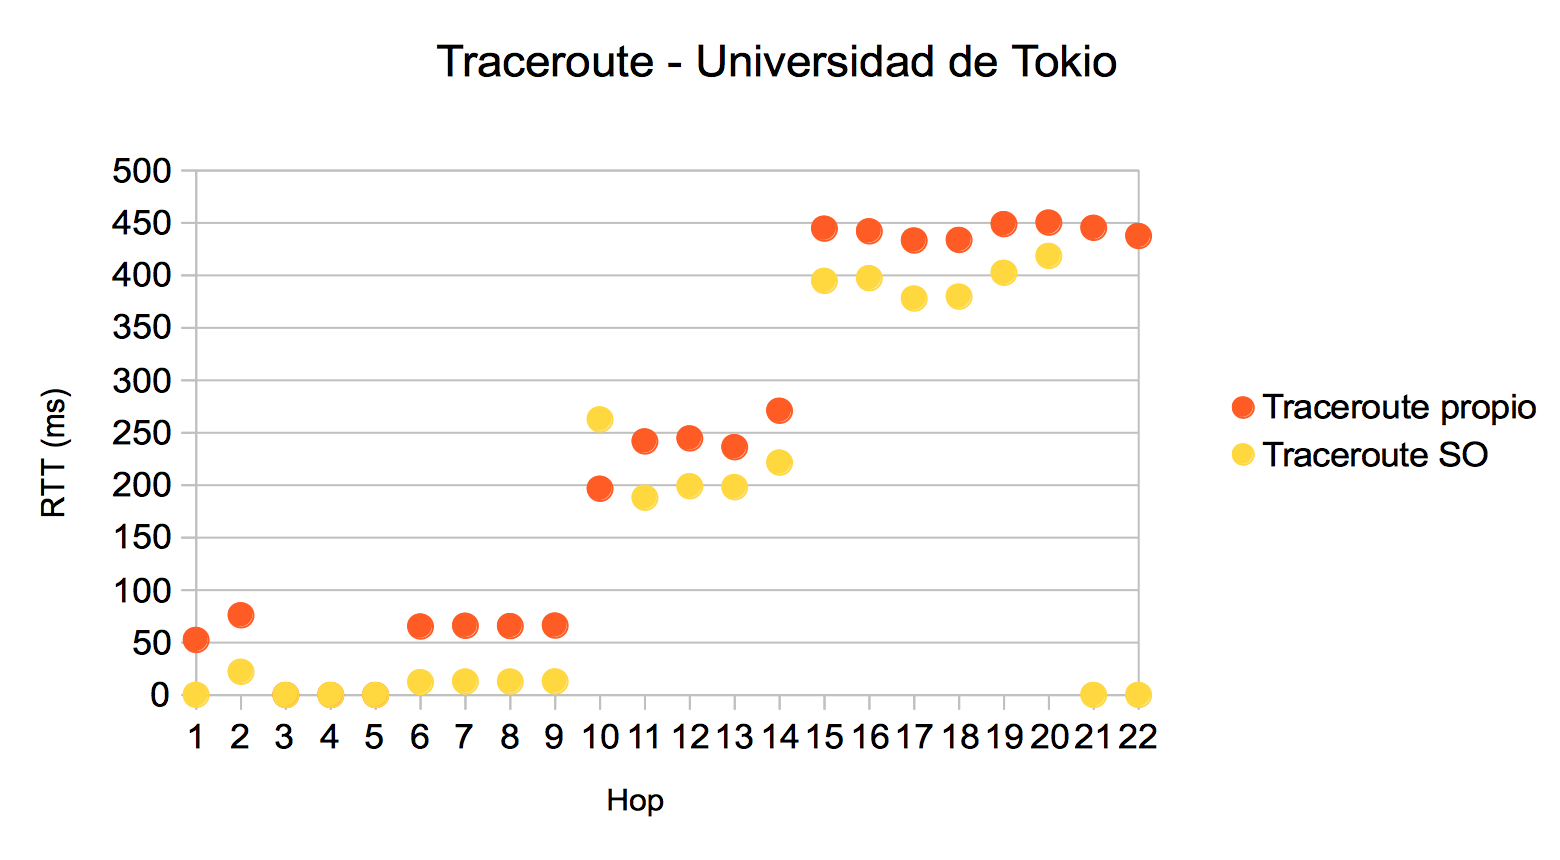
\includegraphics[width=1\textwidth]{imagenes/1ra_parte/Japon_1ergrafico.png}}

Se cumple en este ejemplo, que muchos de los hops intermedios al host final, no responden al pedido. Esto presenta dificultadades en el analisis de los datos. 

\centerline{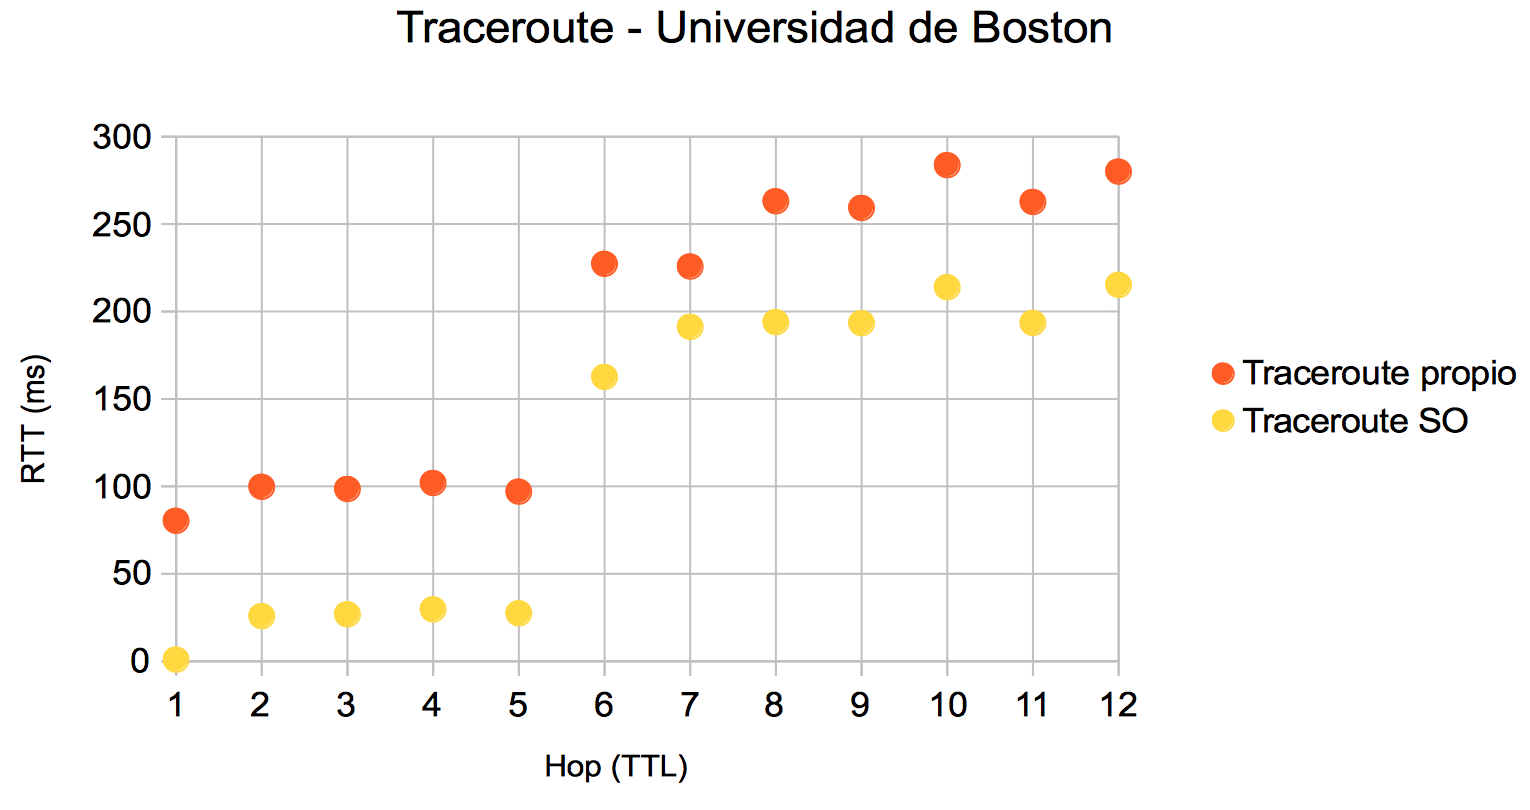
\includegraphics[width=1\textwidth]{imagenes/1ra_parte/EEUU_1ergrafico.png}}

El análisis de los datos obtenidos para cada herrmienta y los gráficos presentados, permitieron obtener diversas conclusiones con respecto al comportamiento de los paquetes en las distintas redes. Estos comportamientos se ven reflados en los tiempos de RTT que presenta cada paquete para cada TTL. A continuación enumeranemos los escenarios que se pudieron encontrar y que generan inconsistencias en las mediciones:

\begin{itemize}
\item Existe más de un ruta posible para un cierto número de TTL para un mismo host de destino. En el caso de la herramienta de traceroute desarrollada por nosotros, no se distingue por host sino por número de TTL. Es decir, el promedio de RTT obtenido a partir de mil paquetes enviados con una misma IP destino y TTL, se realizará sin distinguir si la dirección IP correspondiente a la respuesta es siempre el mismo. Existe una amplia red de routers intermedios que se pueden utilizar para llegar a un mismo destino. En el caso del traceroute brindado por el sistema operativo, se realiza el promedio sobre únicamente tres paquetes diferentes, dándose mayormente que tengan la misma dirección IP. 

\item Hay host intermedios a un destino final que pueden no responder a un ping enviado. Esto puede deberse a que los mismos no estan configurados para responder a este tipo de pedido o que esten congestionados de manera tal de no llegar a responder a tiempo. En el primer caso, no importa la herramienta que se utilice, el resultado siempre será el mismo. Pero, para el segundo escenario planteado, la herramienta brindada por el sistema operativo no intenta resolver la problemática. Sin embargo, en la desarrollada para este trabajo práctico, se basa en el envío de mil paquetes a un mismo TTL, es decir, que el congestionamiento del host podrá liberarse para alguno de los pedidos y la respuesta llegará antes del time out, pudiendose así obtener un RTT estimado. El RTT promedio obtenido del envío de los mil paquetes descarta aquellos que tuvieron time-out para así no disminuir el valor final.

\item Un caso que no es contemplado en ninguno de las dos herramientas utilizadas, es que la ruta que siga un paquete, pasando por una determinada cantidad de hops, no sea siempre la misma. Para el cálculo de los RTT no se contempla que una ruta pueda tomar más tiempo que otra, ya que no se tiene forma de saber cual es el camino exacto que realiza un mensaje para llegar a un determinado hop intermedio. En el caso de la herramienta desarrollada se simula el paso del paquete por distintos host hasta llegar el de la universidad deseada, pero con respecto a los RTT de los hop intermedios, se los trata sin distinguir la ruta que realizan. 
\end{itemize}



Uno de los motivos que afecta a los tiempos en los que un paquete tarda en llegar a un host y luego retornar, es el del congestionamiento que puede existir en la red. El mismo surge a partir de un alto número de paquetes existentes en la misma, debido a un gran número de personas que intentan conectarse a un mismo lugar. Para poder observar este comportamiento, es decir, los fluctuantes valores de RTT para cada hop intermedio, se realizó el siguiente experimento, el cual consiste en analizar el tráfico de la red en distintas horas del día. Para ello se ejecutó el traceroute desarrollado en tres horarios diferentes. 

En primer lugar se presenta la Universidad Humboldt de Berlín. 

%\centerline{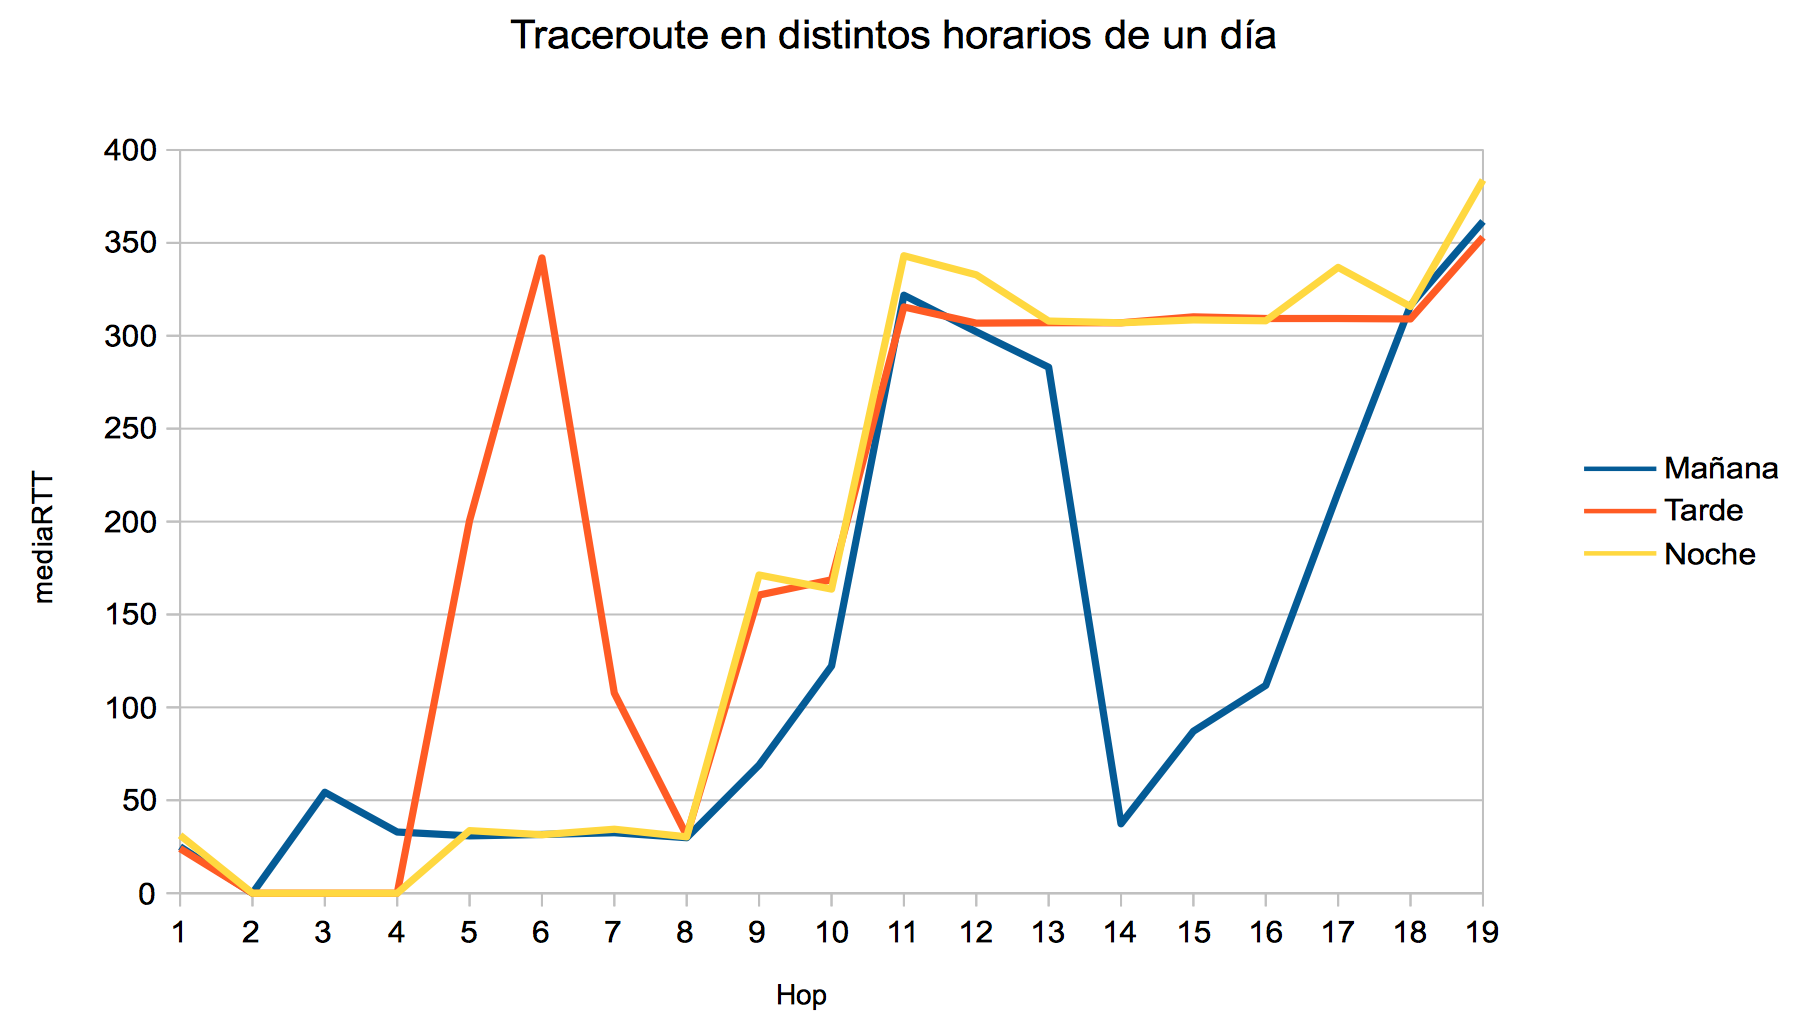
\includegraphics[width=0.9\textwidth]{imagenes/1ra_parte/trace_distintos_horarios_alemania.png}}

El siguiente diagrama corresponde a los valores de RTT obtenido para cada TLL con destino final la Universidad de Moscú.

\centerline{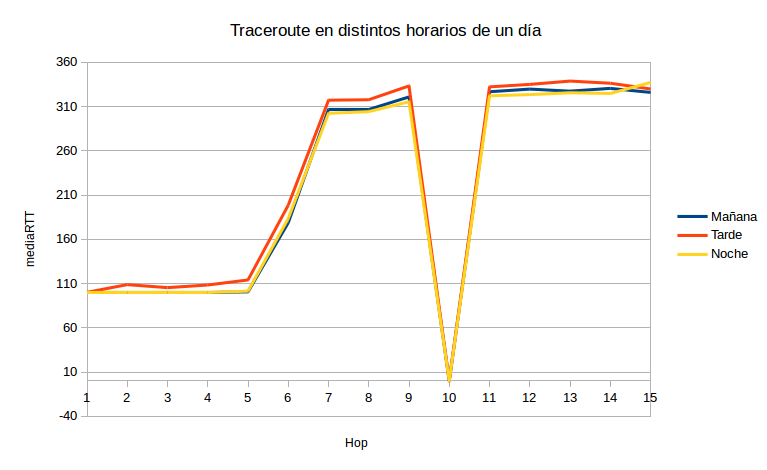
\includegraphics[width=0.9\textwidth]{imagenes/1ra_parte/trace_distintos_horarios_rusia.png}}

A continuación se presenta el caso de la Universidad de Tokio.

\centerline{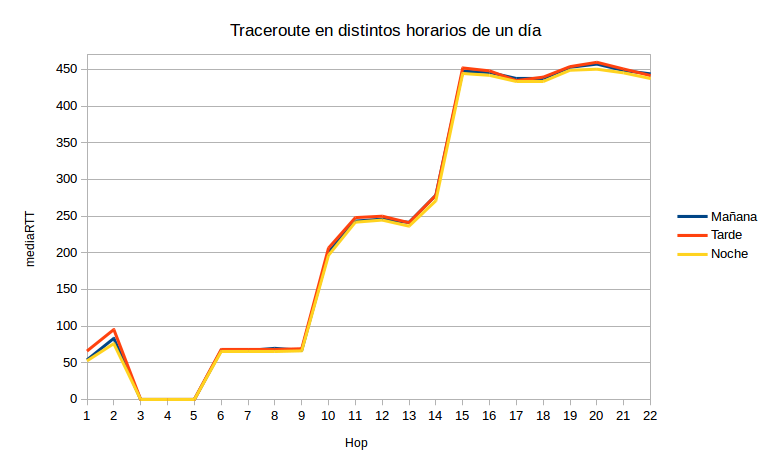
\includegraphics[width=0.9\textwidth]{imagenes/1ra_parte/trace_distintos_horarios_japon.png}}

Finalmente, los valores obtenidos para la Universidad de Boston. 

\centerline{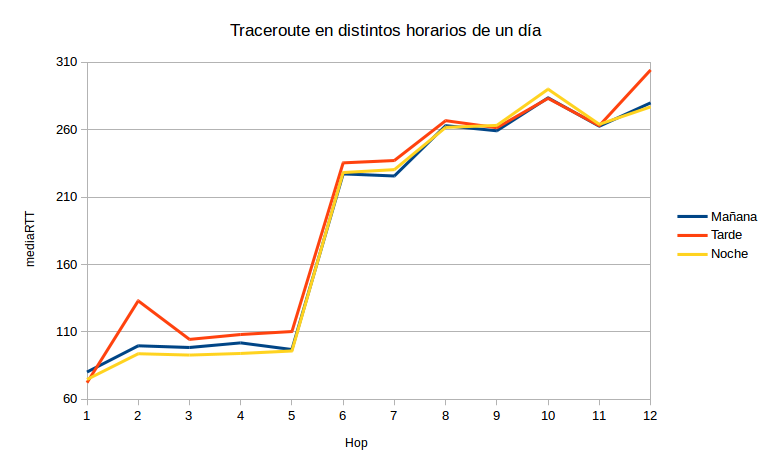
\includegraphics[width=0.9\textwidth]{imagenes/1ra_parte/trace_distintos_horarios_eeuu.png}}

Se puede observar que dependiendo del horario en el que se realiza la medición, algunos RTT para hop intermedios, presentan una diferencia importante con respecto a los de otros momentos del día. 


Luego, para continuar con el análisis de la red, se agrega a la herramienta desarrollada por nosotros un agregado para que se calcule el valor standard (ZRTT) de cada salto con respecto a la ruta global. El cálculo a realizarse es el siguiente:

 \begin{equation}
 	ZRTT_i = \frac{RTT_i - \overline{RTT}}{SRTT} 
 \end{equation}

 Siendo RTT$_{i}$ el RTT medido para el salto entre host número i, $\overline{RTT}$ el promedio para los RTT de todos los saltos realizados y por último el SRTT representa el desvío standard de los RTTs de la ruta, y se calcula de la siguiente manera:

\begin{equation}
 	SRTT = \sqrt{\frac{1}{n} \sum_{i=1}^{n} (RTT_i - \overline{RTT})^2}
 \end{equation}

El ZRTT nos permite definir de forma rápida y exacta cuánto se aleja un RTT de un salto específico respecto al promedio. Luego se podrán realizar diversos análisis y conclusiones utilizando los valores obtenidos en los siguientes gráficos. Estos últimos representan el ZRTT calculado para una medición hecha con mil paquetes para cada TTL con destino cada una de las universidades definidas previamente. 

\centerline{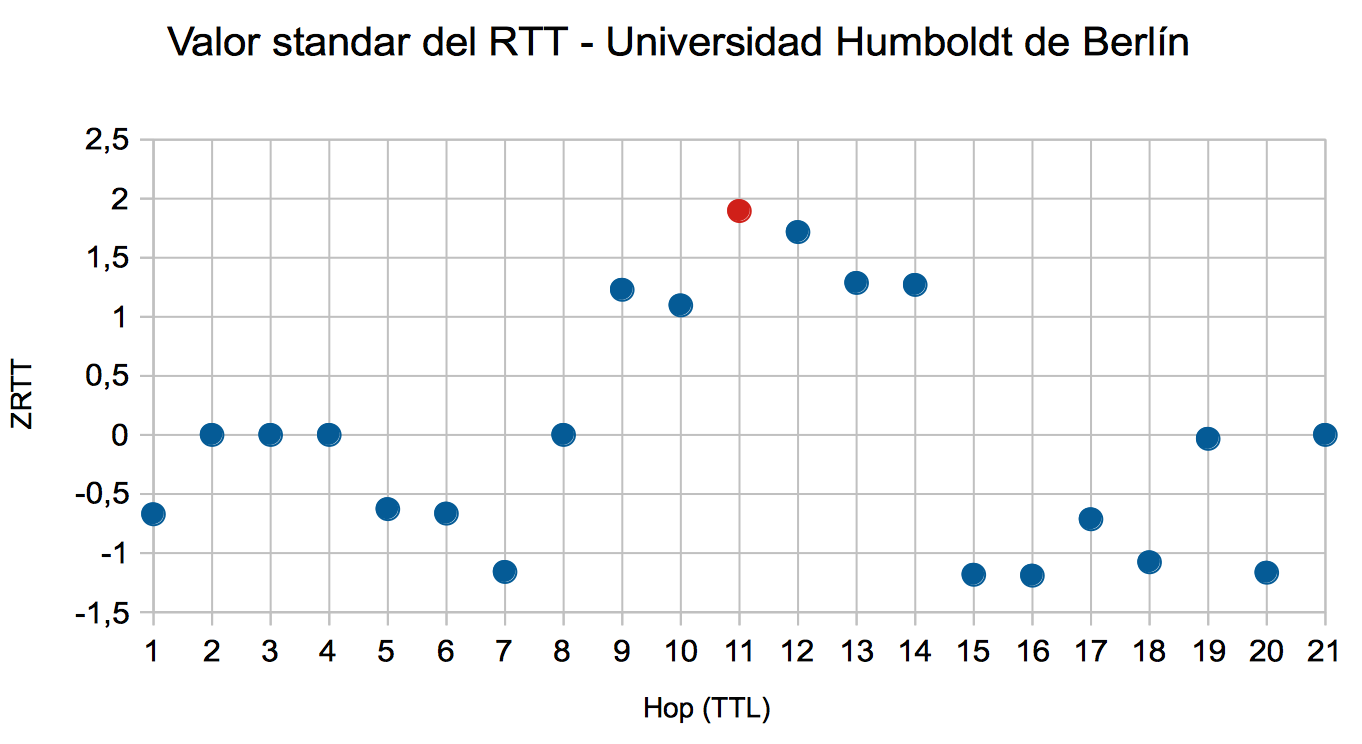
\includegraphics[width=0.8\textwidth]{imagenes/1ra_parte/Alemania_3ergrafico.png}}

\centerline{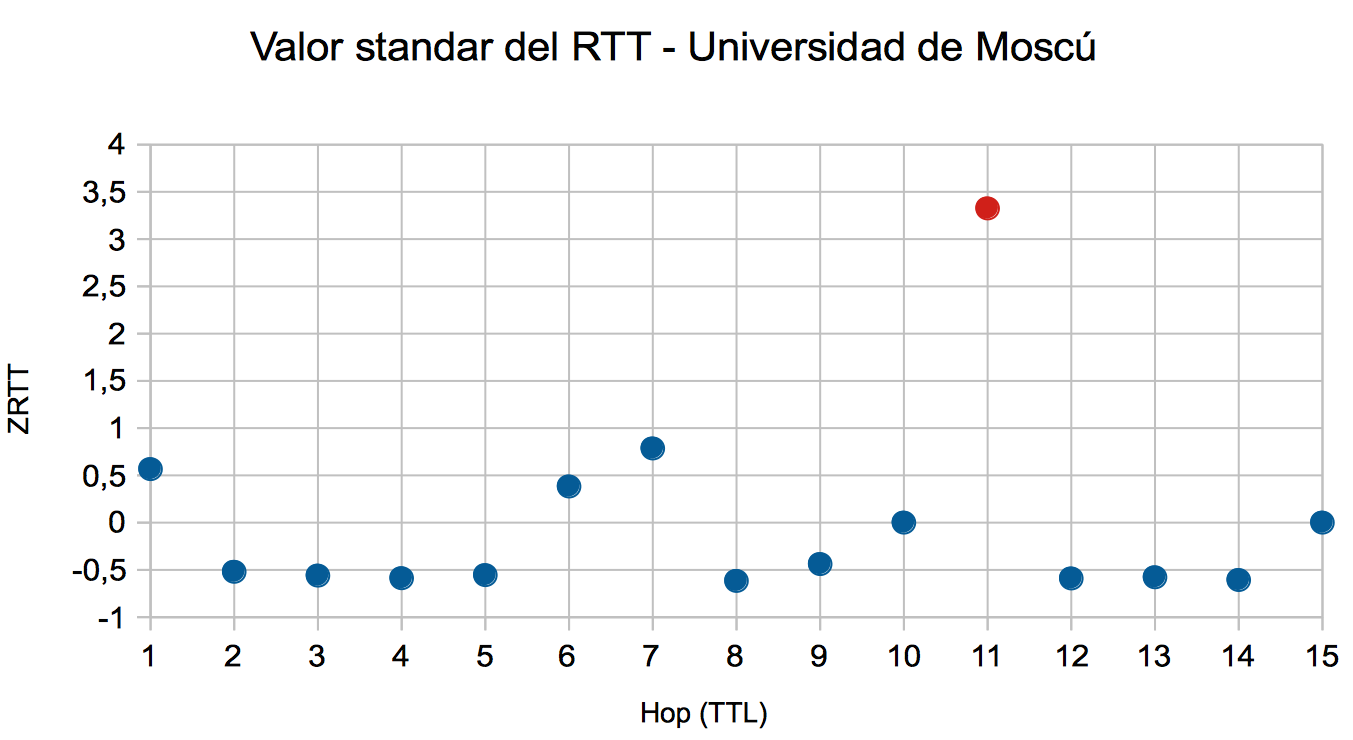
\includegraphics[width=0.8\textwidth]{imagenes/1ra_parte/Rusia_3ergrafico.png}}

\centerline{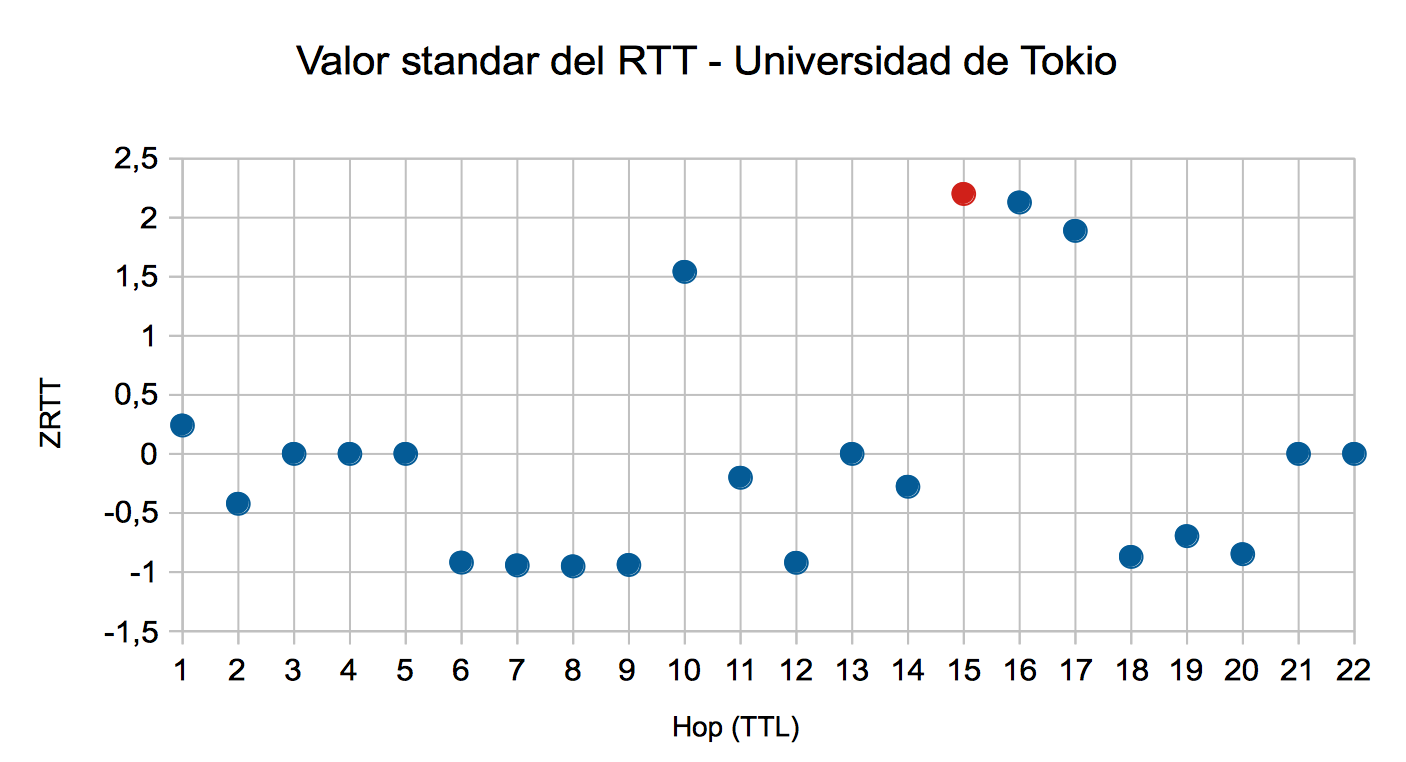
\includegraphics[width=0.8\textwidth]{imagenes/1ra_parte/Japon_3ergrafico.png}}

\centerline{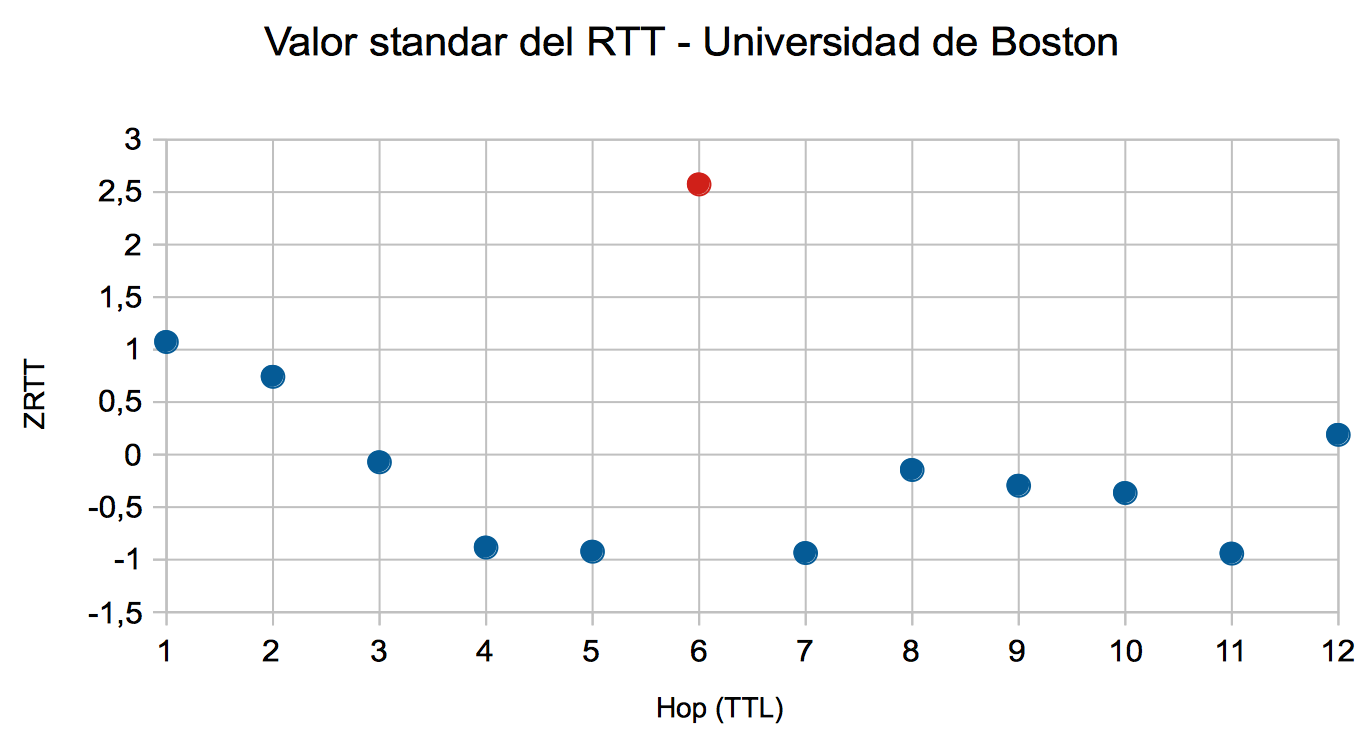
\includegraphics[width=0.8\textwidth]{imagenes/1ra_parte/EEUU_3ergrafico.png}}


\newpage
\section{Gráficos y análisis}

En esta parte del trabajo práctico se requiere determinar los enlaces transatlánticos que utiliza un paquete para llegar a destino. Estos enlaces se caracterizan por atravezar el Atlántico, por lo tanto poseen ciertas propiedades que los diferencian de los demás. Para poder detectar los posibles enlaces se utilizan las mediciones realizadas en la seeción anterior. A partir de los valores que se obtienen al ir recorriendo cada enlace por el que pasa una señal se puede determinar donde se encuentra el mayor salto.
Utilizandose el ZRTT calculado para cada salto se puede definir cuales son los valores que se encuentran más alejados del promedio, por lo tanto, aquellos que cumplan esa condición, serán los que representen el cambio de continente, habíendose atravezado el Atlántico.

Un ejemplo de cuando no funciona la metodología presentada, es aquel paquete que no utiliza por ningún enlace transatlántico. Determinaremos como trasatlánticos a aquel que no corresponda, ya que nos basamos en los tiempos transcurridos entre cada hops, por lo tanto no interesa si pasó o no por algún enlace específico.


\centerline{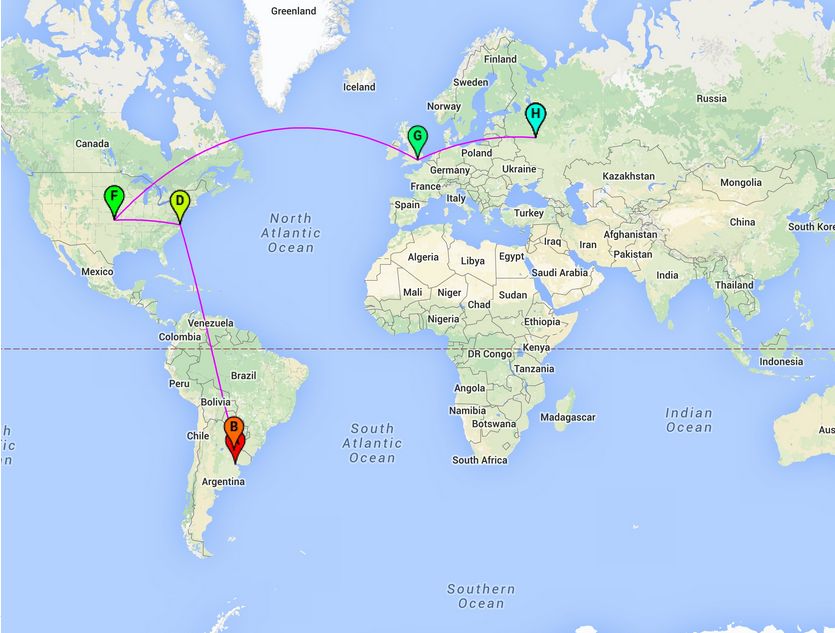
\includegraphics[width=0.8\textwidth]{mapas/rusia.png}}

\begin{center}
 \begin{tabular}{|l|l|l|l|l|}
    \hline
    Hop &Dirección IP &País &Ciudad &Lat - Long \\ \hline \hline
    1 &  & & & \\ \hline
    2 &  & & & \\ \hline
    3 &  & & & \\ \hline
    4 &  & & & \\ \hline
    5 &  & & & \\ \hline
    6 &  & & & \\ \hline
    7 &  & & & \\ \hline
    8 &  & & & \\ \hline
    9 &  & & & \\ \hline
    10 & & & & \\ \hline
    11 & & & & \\ \hline
    12 & & & & \\ \hline
    13 & & & & \\ \hline
    14 & & & & \\ \hline
    15 & & & & \\ \hline
    16 & & & & \\ \hline
    17 & & & & \\ \hline
 \end{tabular}
\end{center}

De acuerdo a la heurística desarrollada, el enlace trasatlántico se encuentra el marcador con la letra $CUAL$, y corresponde al que se encuentra entre el hop $NUMERO$ y el $NUMERO$.

\centerline{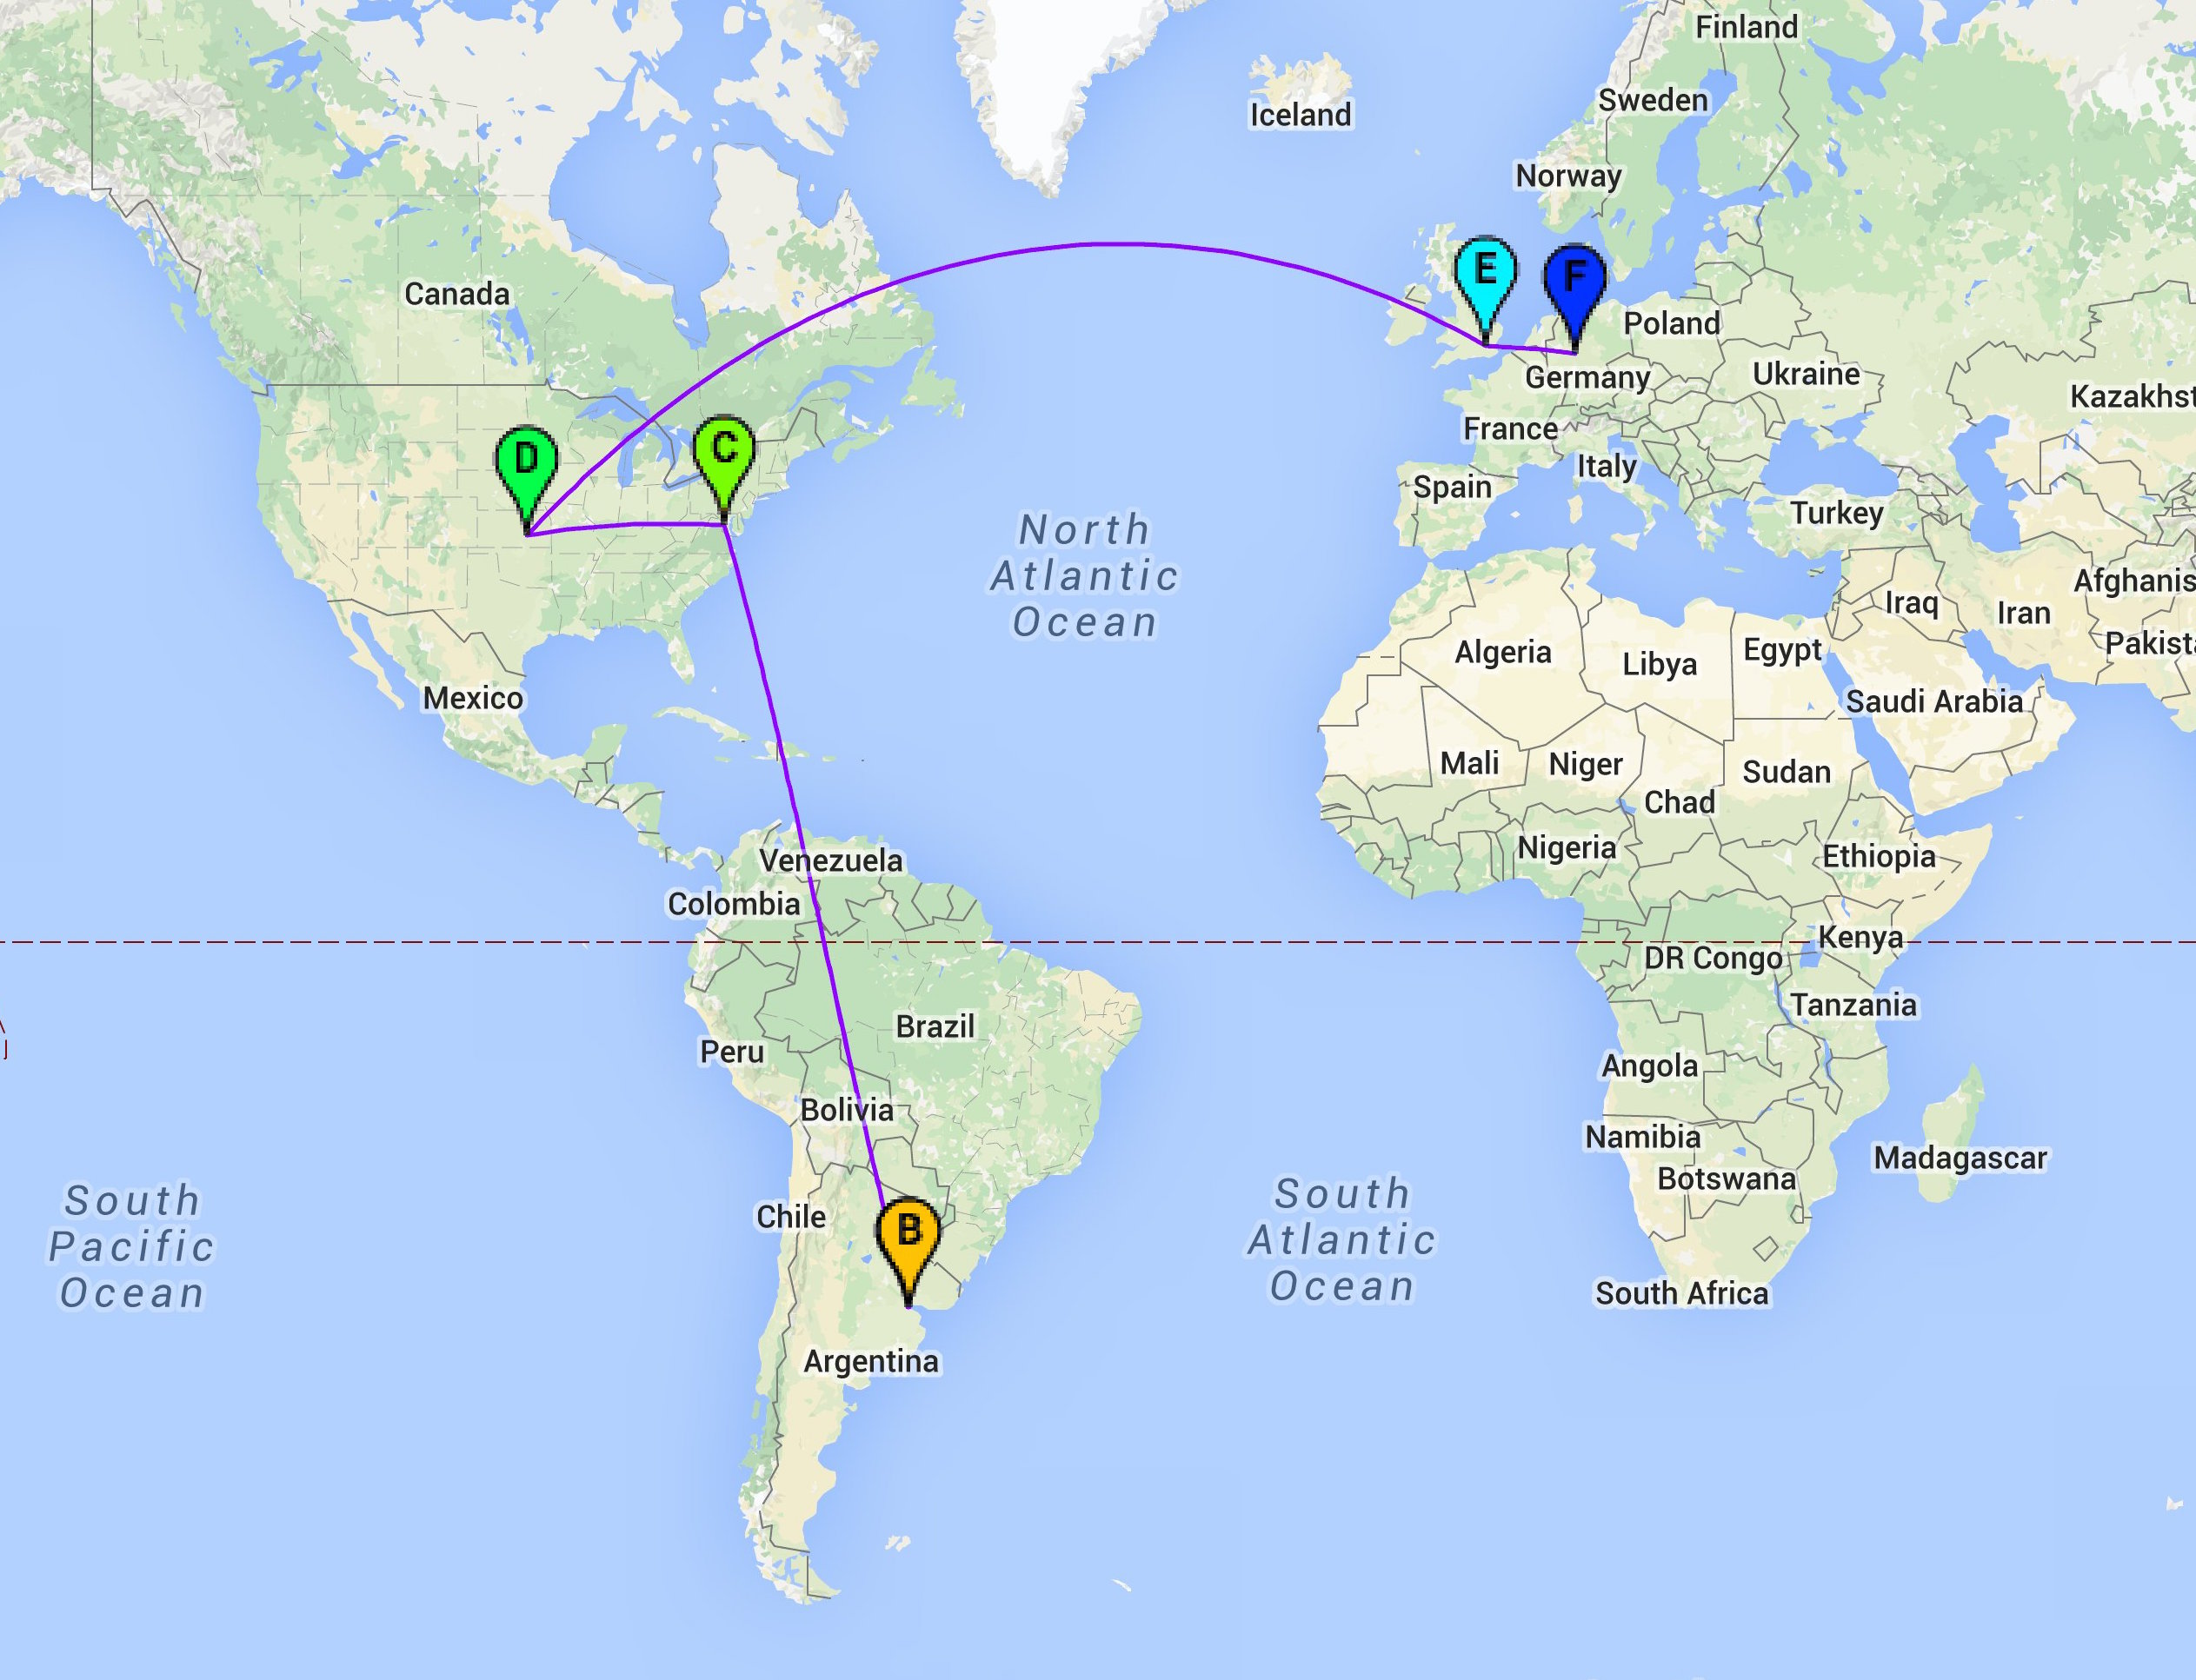
\includegraphics[width=0.8\textwidth]{mapas/Alemania.jpeg}}

\begin{center}
 \begin{tabular}{|l|l|l|l|l|}
    \hline
    Hop &Dirección IP &País &Ciudad &Lat - Long \\ \hline \hline
    1 & 190.190.247.1 & Argentina & Buenos Aires & -34.6 -58.5333	\\ \hline
    2 & 200.89.165.173 & Argentina & Buenos Aires & -34.6 -58.5333	\\ \hline
    3 & 200.89.165.130 & Argentina & Buenos Aires & -34.6 -58.5333	\\ \hline
    4 & 200.89.165.222 & Argentina & Buenos Aires & -34.6 -58.5333	\\ \hline
    5 & 208.178.195.205 & United States & Alexandria & 38.8048 -77.0469 \\ \hline
    6 & 67.17.75.66 & United States & - & 38.0 -97.0 \\ \hline
    7 & 4.68.111.121 & United States & - & 38.0 -97.0 \\ \hline
    8 & 4.68.111.121 & United States & - & 38.0 -97.0 \\ \hline
    9 & 4.69.154.137 & United States & - & 38.0 -97.0 \\ \hline
    10 & 212.162.4.6 & United Kingdom & - &  51.5 -0.13 \\ \hline
    11 & 188.1.144.101 & Germany & - & 51.0 9.0 \\ \hline
    12 & 188.1.144.185 & Germany & - & 51.0 9.0 \\ \hline
    13 & 188.1.144.158 & Germany & - & 51.0 9.0 \\ \hline
    14 & 188.1.144.13 & Germany & - & 51.0 9.0 \\ \hline
    15 & 188.1.144.17 & Germany & - & 51.0 9.0 \\ \hline
    16 & 188.1.236.70 & Germany & - & 51.0 9.0 \\ \hline
    17 & 141.20.0.210 & Germany & Berlin & 52.5167 13.4 \\ \hline
 \end{tabular}
\end{center}

En este caso se considera, observando el mapa, como enlace trasatlántico aquel que ocurre entre el hop $9$ y el $10$. Se puede observar en comparación con las variaciones de los valores de ZRTT, que el correspondiente al hop $10$, presenta un valor alto con respecto a los previos. Esto demuestra que el ZRTT es efectivo al momento de definir los saltos con cambios de continentes y que atraviezan el Atlántico.


\centerline{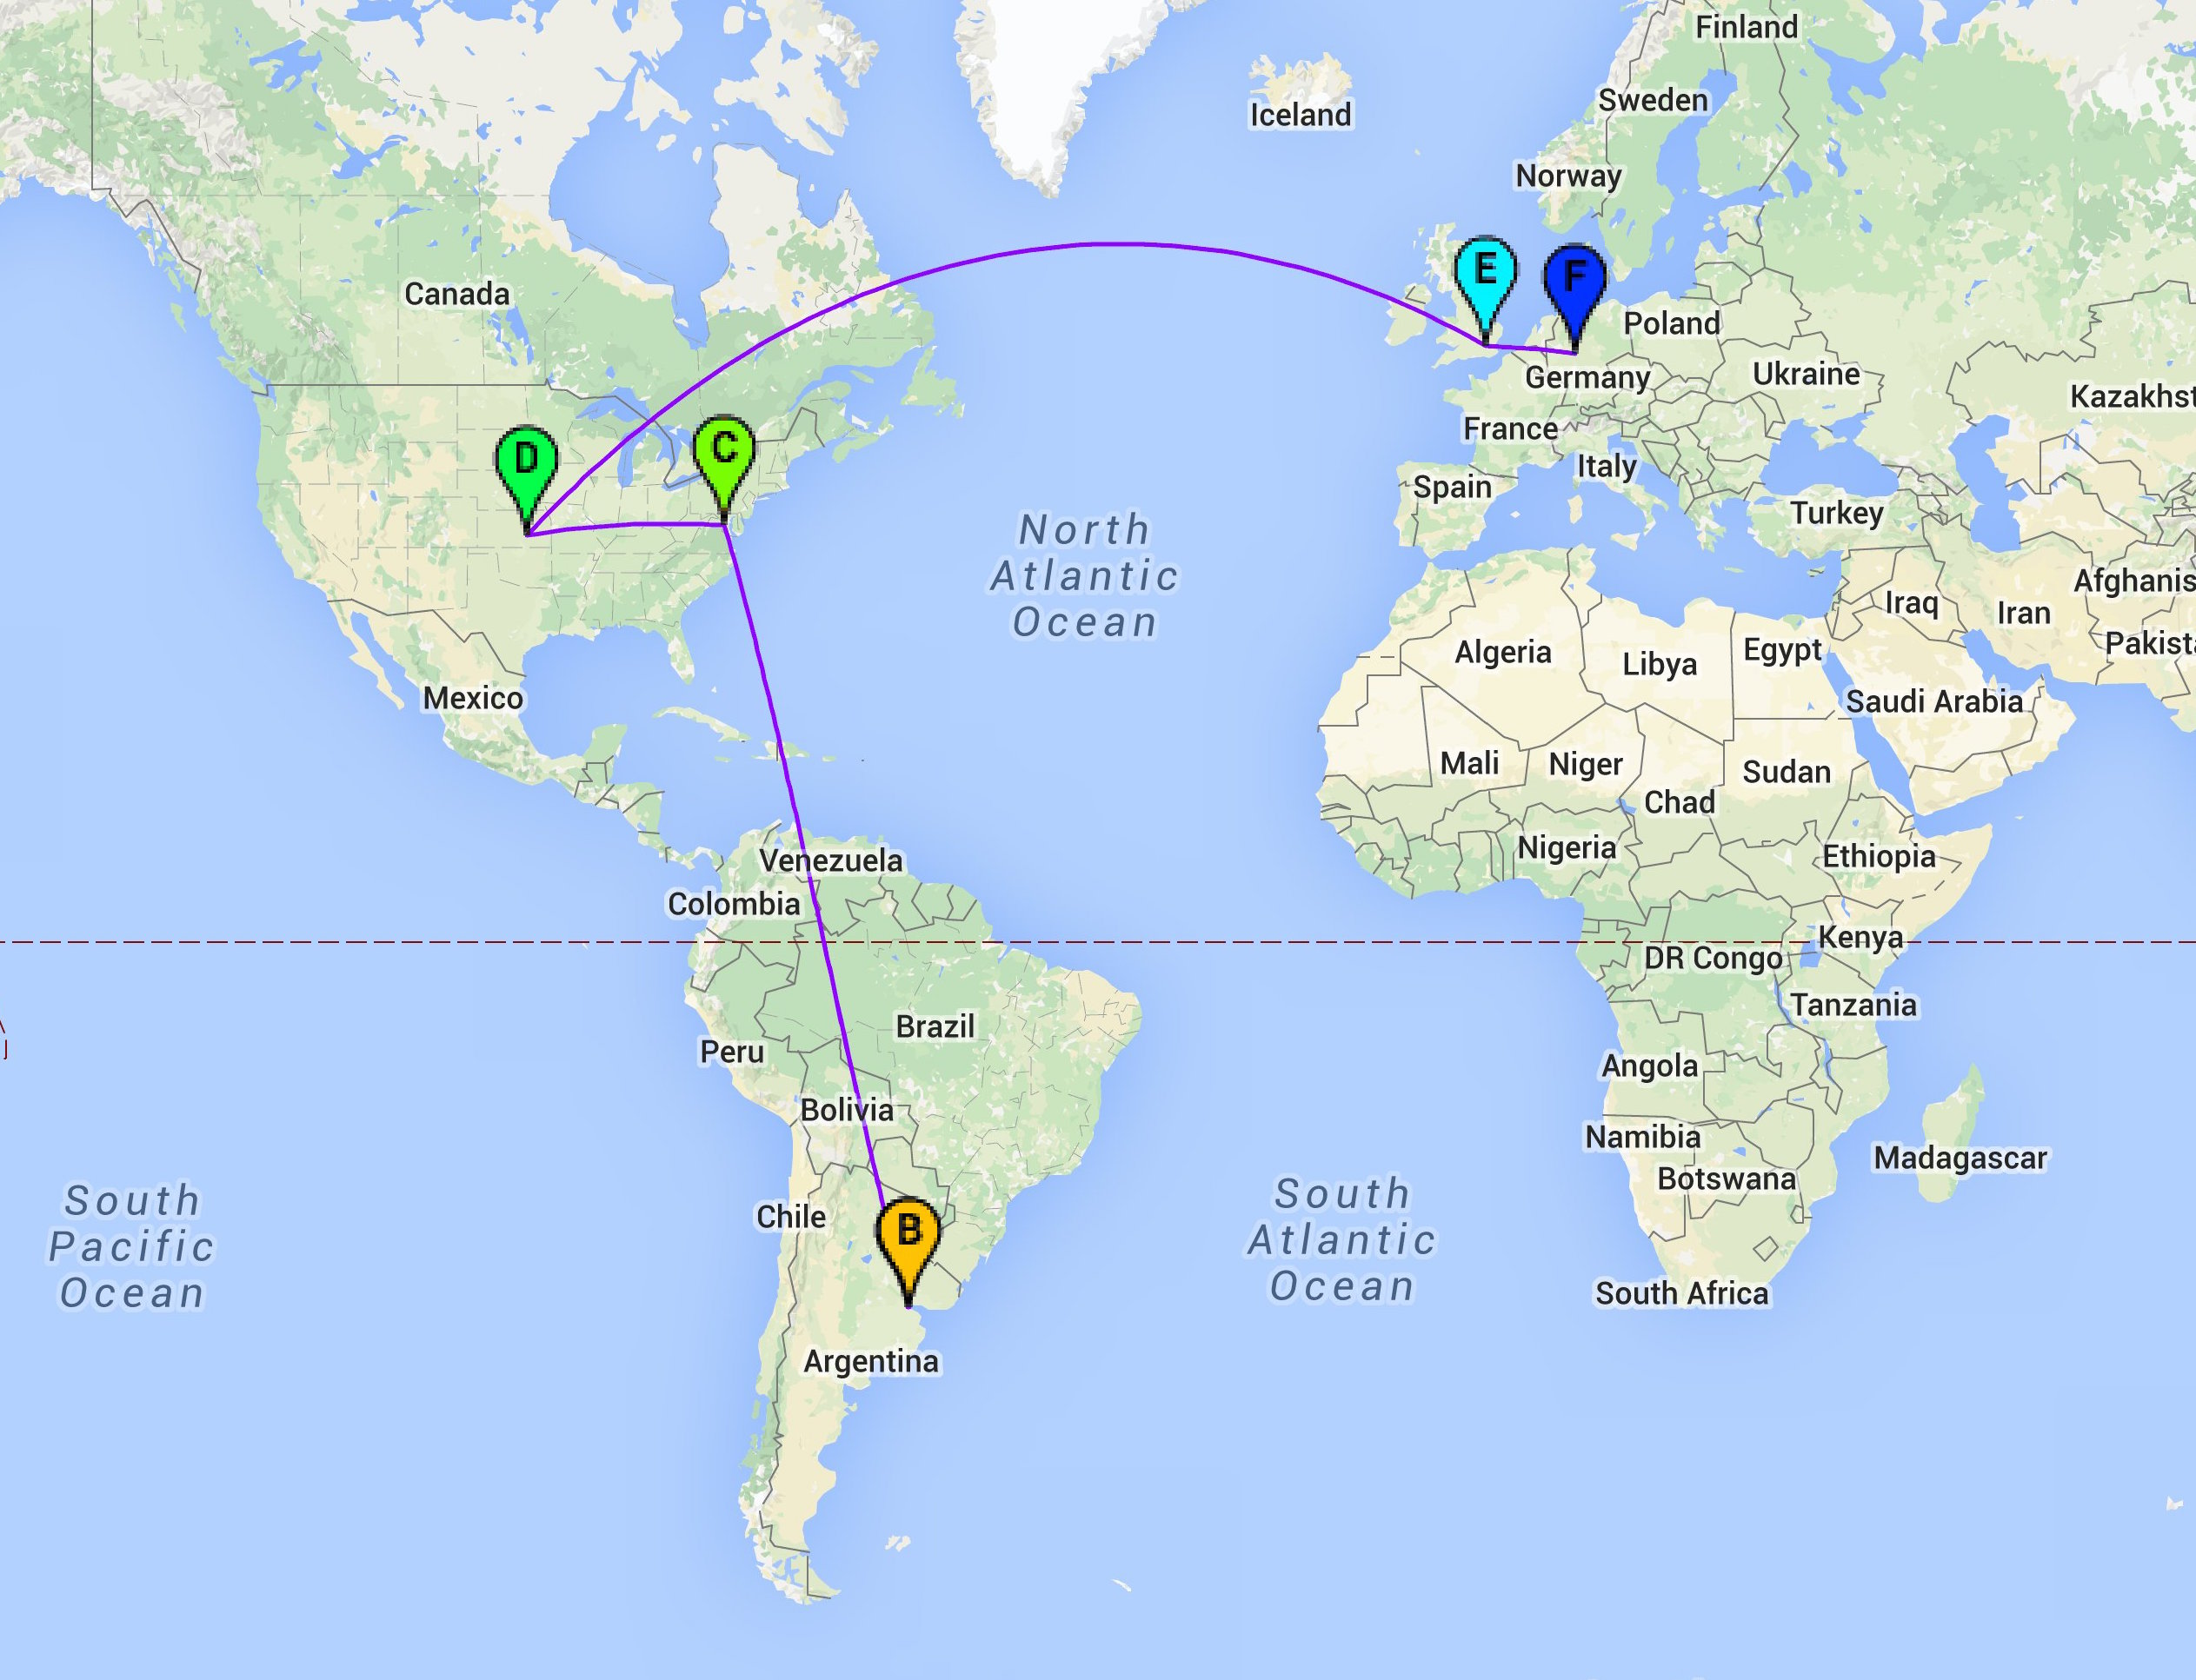
\includegraphics[width=0.8\textwidth]{mapas/Alemania.jpeg}}

\begin{center}
 \begin{tabular}{|l|l|l|l|l|}
    \hline
    Hop &Dirección IP &País &Ciudad &Lat - Long \\ \hline \hline
    1 &  & & & \\ \hline
    2 &  & & & \\ \hline
    3 &  & & & \\ \hline
    4 &  & & & \\ \hline
    5 &  & & & \\ \hline
    6 &  & & & \\ \hline
    7 &  & & & \\ \hline
    8 &  & & & \\ \hline
    9 &  & & & \\ \hline
    10 & & & & \\ \hline
    11 & & & & \\ \hline
    12 & & & & \\ \hline
    13 & & & & \\ \hline
    14 & & & & \\ \hline
    15 & & & & \\ \hline
    16 & & & & \\ \hline
    17 & & & & \\ \hline
 \end{tabular}
\end{center}

\centerline{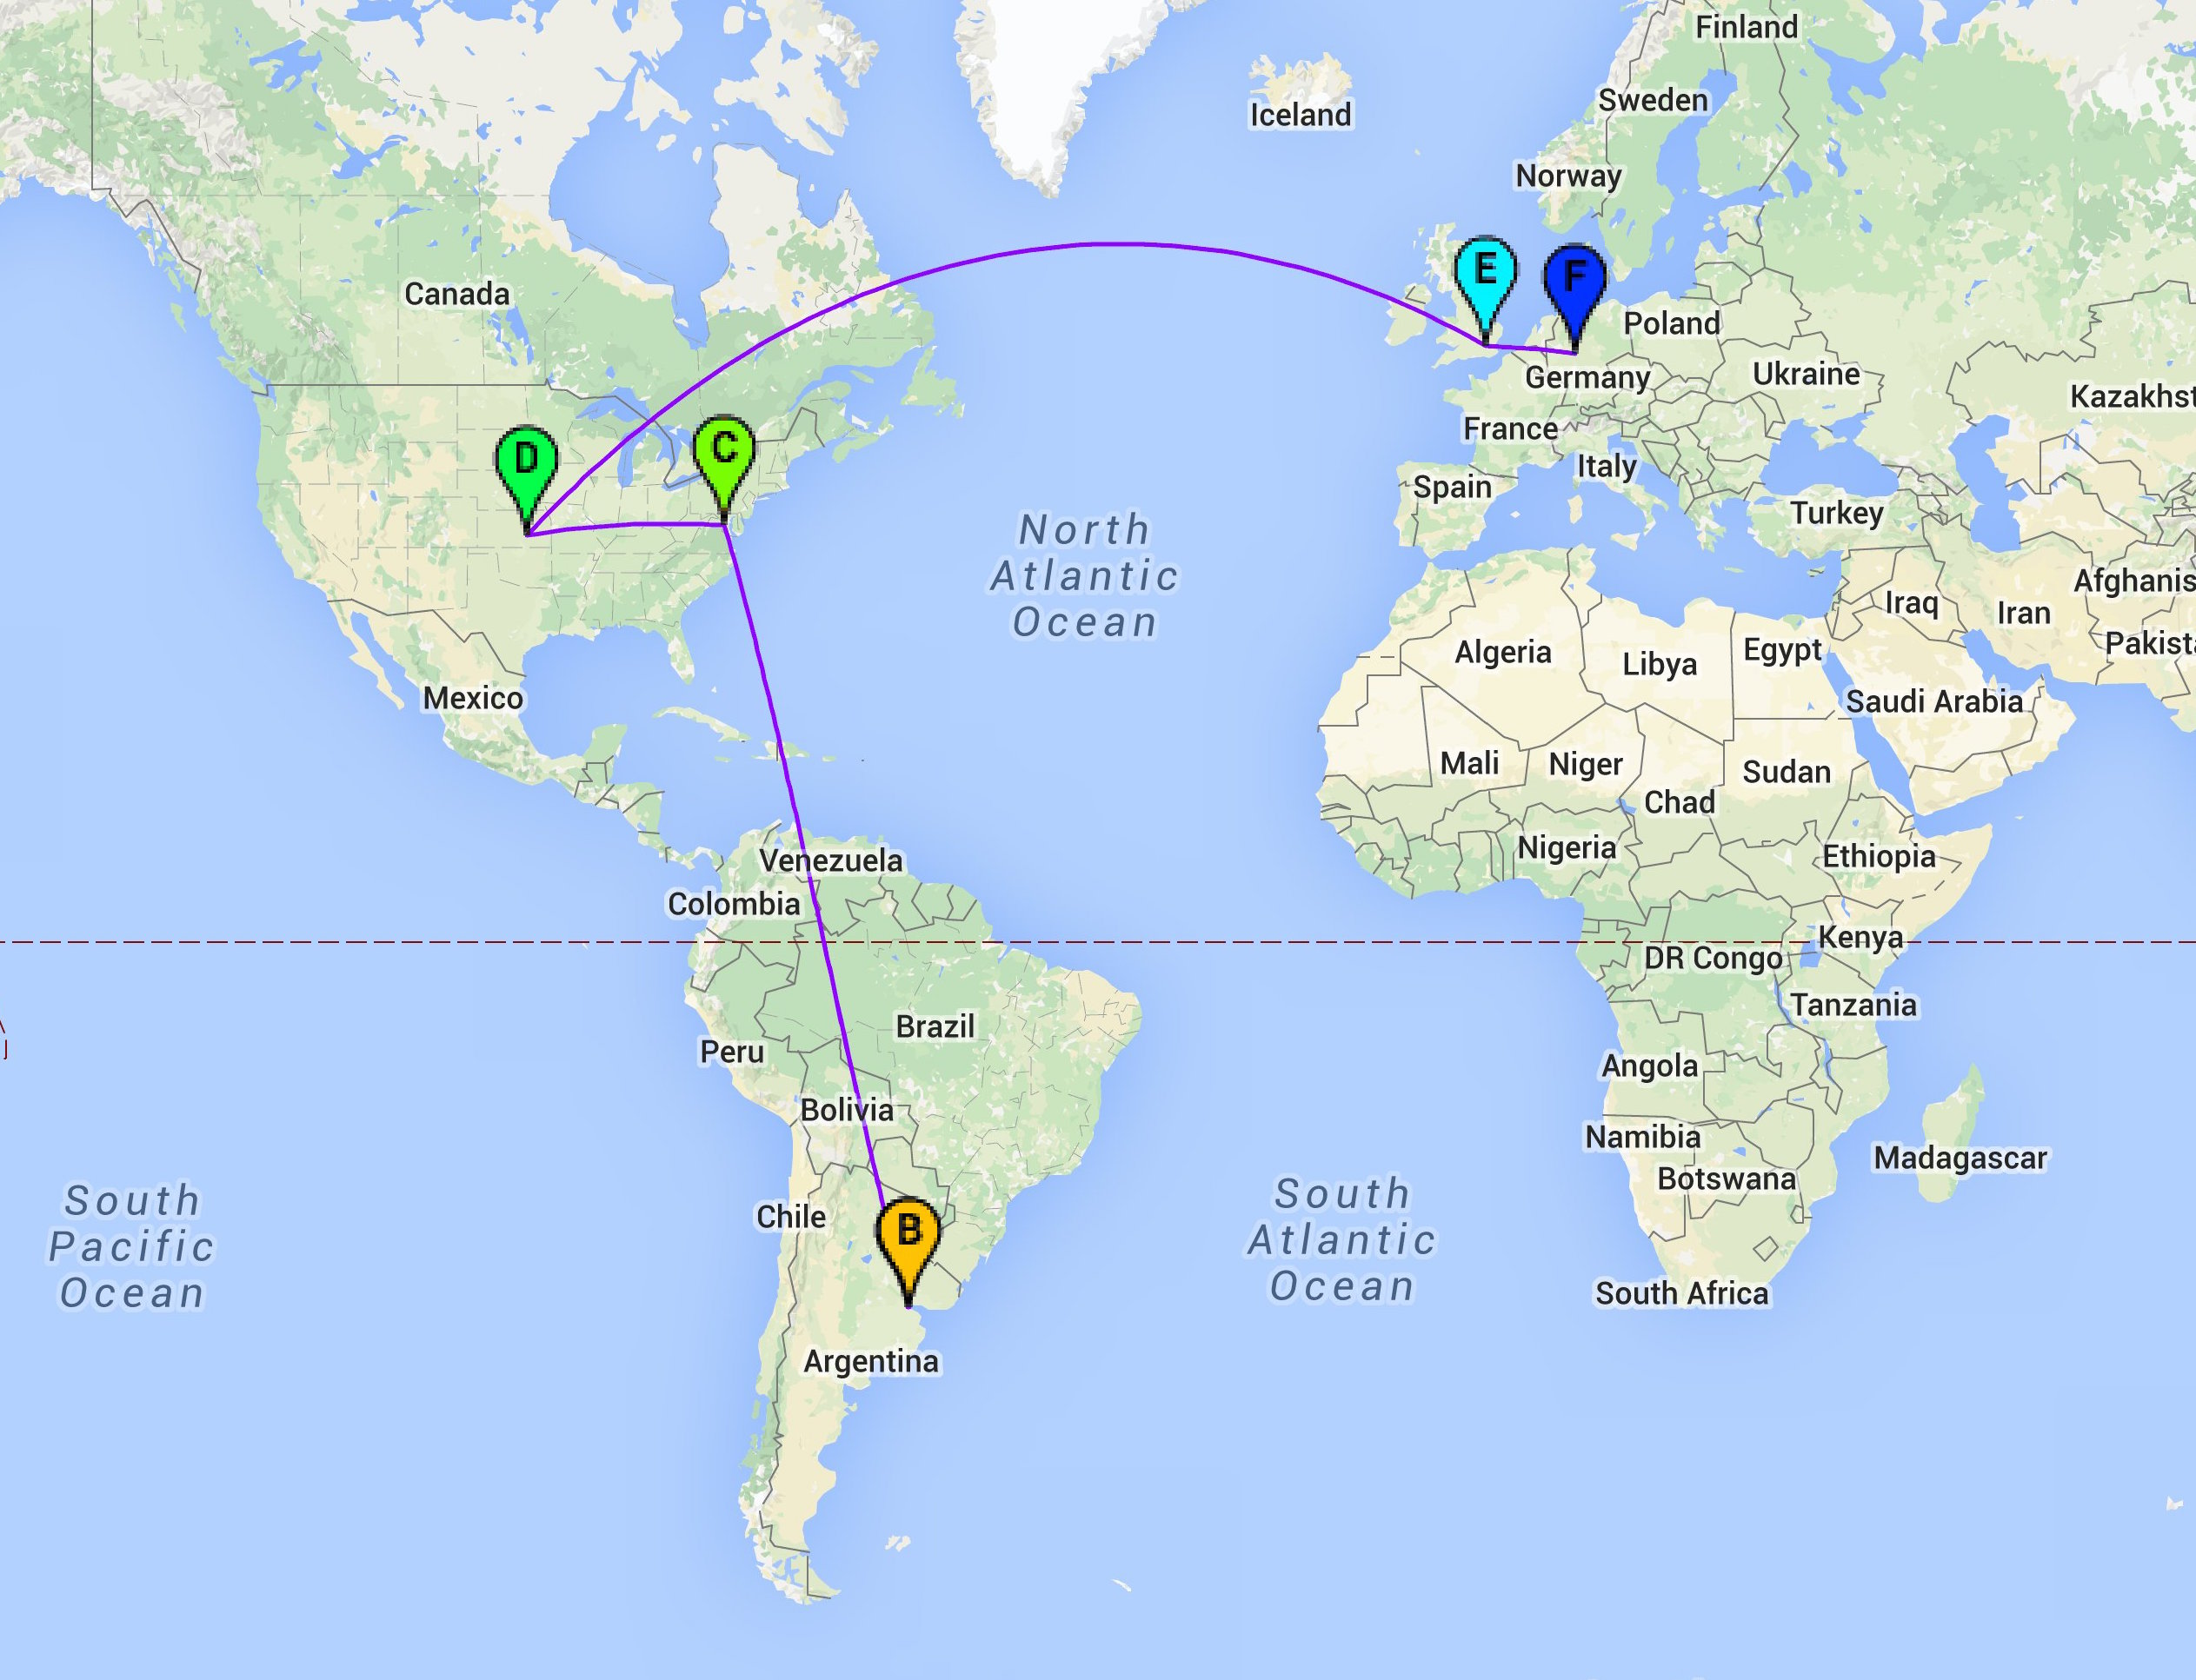
\includegraphics[width=0.8\textwidth]{mapas/Alemania.jpeg}}

\begin{center}
 \begin{tabular}{|l|l|l|l|l|}
    \hline
    Hop &Dirección IP &País &Ciudad &Lat - Long \\ \hline \hline
    1 &  & & & \\ \hline
    2 &  & & & \\ \hline
    3 &  & & & \\ \hline
    4 &  & & & \\ \hline
    5 &  & & & \\ \hline
    6 &  & & & \\ \hline
    7 &  & & & \\ \hline
    8 &  & & & \\ \hline
    9 &  & & & \\ \hline
    10 & & & & \\ \hline
    11 & & & & \\ \hline
    12 & & & & \\ \hline
    13 & & & & \\ \hline
    14 & & & & \\ \hline
    15 & & & & \\ \hline
    16 & & & & \\ \hline
    17 & & & & \\ \hline
 \end{tabular}
\end{center}


\begin{center}
 \begin{tabular}{|l|l|l|l|l|l|}
    \hline
    Hop &Dirección IP &País &Ciudad &ISP &Lat - Long \\ \hline \hline
    3 & 181.47.254.85 & Argentina & - & Telecentro S.A. & -34.6033 -58.3817 \\ \hline
    4 & 208.178.195.214 & United States & Virginia & Level 3 Communications, Inc. & 36.8267 -76.0179 \\ \hline
    5 & 208.178.195.213 & United States & Virginia & Level 3 Communications, Inc. & 36.8267 -76.0179 \\ \hline
    6 & 67.17.75.66 & United States  & - & Level 3 Communications, Inc. & 38 -97 \\ \hline
    7 & 4.68.111.121 & United States  & - & Level 3 Communications, Inc. & 38 -97 \\ \hline
    8 & 4.69.140.90 & United States & Florida & Level 3 Communications, Inc. & 25.9372 -80.317 \\ \hline
    9 & 4.53.56.6 & United States & Massachusetts & Level 3 Communications, Inc. & 42.2612 -71.4634 \\ \hline
    10 & 128.197.254.113 & United States & Massachusetts  & Boston University & 42.3451 -71.0993 \\ \hline
    11 & 128.197.254.166 & United States & Massachusetts  & Boston University & 42.3451 -71.0993 \\ \hline
    12 & 128.197.26.34 & United States & Massachusetts  & Boston University & 42.3451 -71.0993 \\ \hline
 \end{tabular}
\end{center}

\centerline{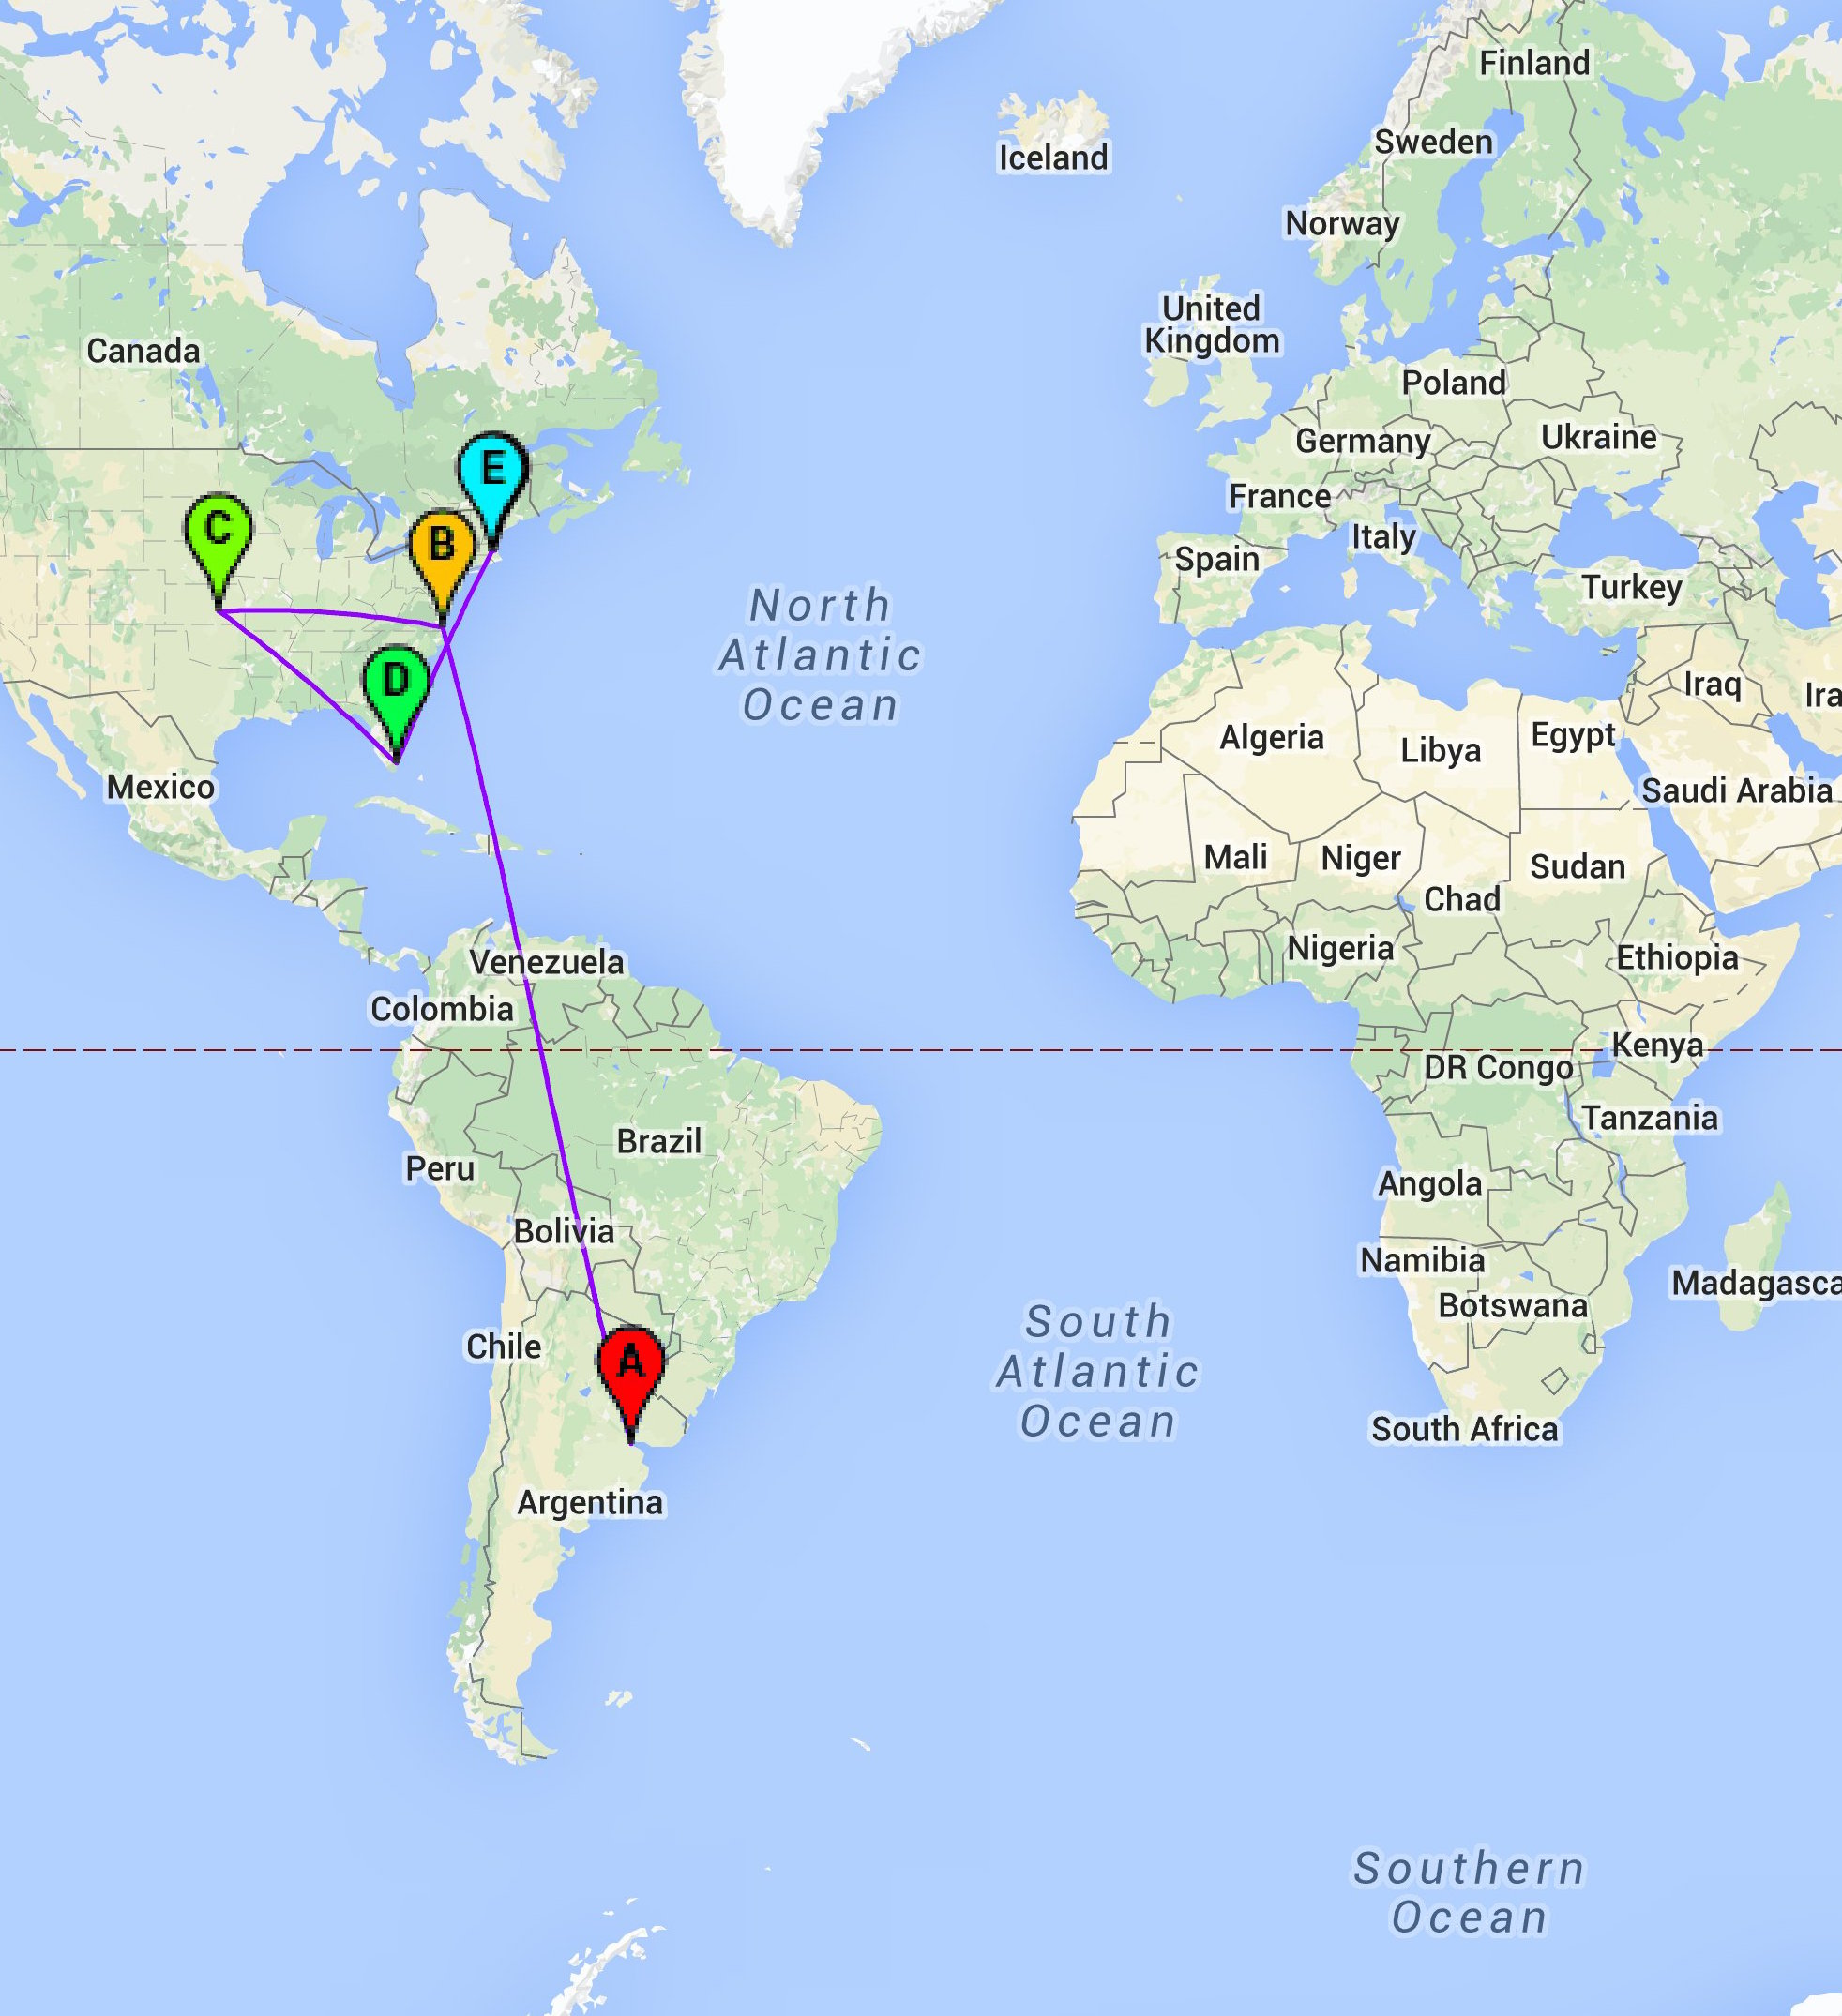
\includegraphics[width=0.8\textwidth]{mapas/EEUU}}

% eeuu noche

\begin{center}
 \begin{tabular}{|l|l|l|l|l|}
    \hline
    Hop &Dirección IP &País &Ciudad &Lat - Long \\ \hline \hline
    3 & 181.47.254.85 & Argentina  & AS27747 & -34.6033 -58.3817 \\ \hline
    4 & 208.178.195.214 & United States & Virginia AS3549 & 36.8267 -76.0179 \\ \hline
    5 & 208.178.195.213 & United States & Virginia AS3549 & 36.8267 -76.0179 \\ \hline
    6 & 67.17.75.66 & United States  & AS3549 & 38 -97 \\ \hline
    7 & 4.68.111.121 & United States  & AS3356 & 38 -97 \\ \hline
    8 & 4.69.140.90 & United States & Florida AS3356 & 25.9372 -80.317 \\ \hline
    9 & 4.53.56.6 & United States & Massachusetts AS3356 & 42.2612 -71.4634 \\ \hline
    10 & 128.197.254.113 & United States & Massachusetts AS111 & 42.3451 -71.0993 \\ \hline
    11 & 128.197.254.166 & United States & Massachusetts AS111 & 42.3451 -71.0993 \\ \hline
    12 & 128.197.26.34 & United States & Massachusetts AS111 & 42.3451 -71.0993 \\ \hline
 \end{tabular}
\end{center}


% alemania mañana

\begin{center}
 \begin{tabular}{|l|l|l|l|l|}
    \hline
    Hop &Dirección IP &País &Ciudad &Lat - Long \\ \hline \hline
	1 & 190.190.247.1 & Argentina & Buenos Aires & -34.5417 -58.5583 \\ \hline
	3 & 200.89.165.173 & Argentina &  & -34.6033 -58.3817 \\ \hline
	4 & 200.89.165.173 & Argentina &  & -34.6033 -58.3817 \\ \hline
	5 & 200.89.165.173 & Argentina &  & -34.6033 -58.3817 \\ \hline
	6 & 200.89.165.130 & Argentina &  & -34.6033 -58.3817 \\ \hline
	7 & 200.89.165.130 & Argentina &  & -34.6033 -58.3817 \\ \hline
	8 & 208.178.195.205 & United States & Virginia & 38.8048 -77.0469 \\ \hline
	9 & 4.68.111.121 & United States &  & 38 -97 \\ \hline
	10 & 4.68.111.121 & United States &  & 38 -97 \\ \hline
	11 & 4.69.154.137 & United States &  & 38 -97 \\ \hline
	12 & 4.69.154.137 & United States &  & 38 -97 \\ \hline
	13 & 188.1.144.101 & Germany &  & 51 9 \\ \hline
	14 & 212.162.4.6 & United Kingdom &  & 51.5 -0.13 \\ \hline
	15 & 188.1.144.101 & Germany &  & 51 9 \\ \hline
	16 & 188.1.144.185 & Germany &  & 51 9 \\ \hline
	17 & 188.1.144.158 & Germany &  & 51 9 \\ \hline
	18 & 188.1.236.70 & Germany &  & 51 9 \\ \hline
	19 & 141.20.0.210 & Germany & Land Berlin & 52.5167 13.4 \\ \hline
 \end{tabular}
\end{center}

% alemania noche

\begin{center}
 \begin{tabular}{|l|l|l|l|l|}
    \hline
    Hop &Dirección IP &País &Ciudad &Lat - Long \\ \hline \hline
	1 & 190.190.247.1 & Argentina & Buenos Aires & -34.5417 -58.5583 \\ \hline
	5 & 200.89.165.173 & Argentina &  & -34.6033 -58.3817 \\ \hline
	6 & 200.89.165.130 & Argentina &  & -34.6033 -58.3817 \\ \hline
	7 & 200.89.165.222 & Argentina &  & -34.6033 -58.3817 \\ \hline
	8 & 208.178.195.205 & United States & Virginia & 38.8048 -77.0469 \\ \hline
	9 & 67.17.75.66 & United States &  & 38 -97 \\ \hline
	10 & 4.68.111.121 & United States &  & 38 -97 \\ \hline
	11 & 4.69.154.137 & United States &  & 38 -97 \\ \hline
	12 & 4.69.154.137 & United States &  & 38 -97 \\ \hline
	13 & 212.162.4.6 & United Kingdom &  & 51.5 -0.13 \\ \hline
	14 & 188.1.144.101 & Germany &  & 51 9 \\ \hline
	15 & 188.1.144.185 & Germany &  & 51 9 \\ \hline
	16 & 188.1.144.158 & Germany &  & 51 9 \\ \hline
	17 & 188.1.144.13 & Germany &  & 51 9 \\ \hline
	18 & 188.1.144.17 & Germany &  & 51 9 \\ \hline
	19 & 188.1.236.70 & Germany &  & 51 9 \\ \hline
	20 & 141.20.0.210 & Germany & Land Berlin & 52.5167 13.4 \\ \hline
	21 & 141.20.5.188 & Germany & Land Berlin & 52.5167 13.4 \\ \hline
 \end{tabular}
\end{center}

% rusia mañana

\begin{center}
 \begin{tabular}{|l|l|l|l|l|}
    \hline
    Hop &Dirección IP &País &Ciudad &Lat - Long \\ \hline \hline
	1 & 192.168.1.1 & - & - & 0 0 \\ \hline
	2 & 10.20.128.1 & - & - & 0 0 \\ \hline
	3 & 181.47.254.33 & Argentina &  & -34.6033 -58.3817 \\ \hline
	4 & 208.178.195.210 & United States & Virginia & 36.8267 -76.0179 \\ \hline
	5 & 208.178.195.209 & United States & Virginia & 36.8267 -76.0179 \\ \hline
	6 & 4.68.111.121 & United States &  & 38 -97 \\ \hline
	7 & 4.69.158.245 & United States &  & 38 -97 \\ \hline
	8 & 4.69.158.245 & United States &  & 38 -97 \\ \hline
	9 & 213.242.110.198 & United Kingdom &  & 51.5 -0.13 \\ \hline
	11 & 194.85.40.229 & Russia &  & 55.75 37.6166 \\ \hline
	12 & 194.190.254.118 & Russia &  & 55.75 37.6166 \\ \hline
	13 & 93.180.0.174 & Russia & Moscow & 55.7522 37.6156 \\ \hline
	14 & 188.44.33.1 & Russia & Moscow & 55.7522 37.6156 \\ \hline
	15 & 188.44.50.103 & Russia & Moscow & 55.7522 37.6156 \\ \hline
 \end{tabular}
\end{center}

% rusia tarde

\begin{center}
 \begin{tabular}{|l|l|l|l|l|}
    \hline
    Hop &Dirección IP &País &Ciudad &Lat - Long \\ \hline \hline
	1 & 192.168.1.1 & - & - & 0 0 \\ \hline
	2 & 10.20.128.1 & - & - & 0 0 \\ \hline
	3 & 181.47.254.33 & Argentina &  & -34.6033 -58.3817 \\ \hline
	4 & 208.178.195.210 & United States & Virginia & 36.8267 -76.0179 \\ \hline
	5 & 208.178.195.209 & United States & Virginia & 36.8267 -76.0179 \\ \hline
	6 & 4.68.111.121 & United States &  & 38 -97 \\ \hline
	7 & 4.69.158.245 & United States &  & 38 -97 \\ \hline
	8 & 4.69.158.245 & United States &  & 38 -97 \\ \hline
	9 & 213.242.110.198 & United Kingdom &  & 51.5 -0.13 \\ \hline
	11 & 194.85.40.229 & Russia &  & 55.75 37.6166 \\ \hline
	12 & 194.190.254.118 & Russia &  & 55.75 37.6166 \\ \hline
	13 & 93.180.0.174 & Russia & Moscow & 55.7522 37.6156 \\ \hline
	14 & 188.44.33.1 & Russia & Moscow & 55.7522 37.6156 \\ \hline
	15 & 188.44.50.103 & Russia & Moscow & 55.7522 37.6156 \\ \hline
 \end{tabular}
\end{center}

% rusia noche

\begin{center}
 \begin{tabular}{|l|l|l|l|l|}
    \hline
    Hop &Dirección IP &País &Ciudad &Lat - Long \\ \hline \hline
	1 & 192.168.1.1 & - & - & 0 0 \\ \hline
	2 & 10.20.128.1 & - & - & 0 0 \\ \hline
	3 & 181.47.254.33 & Argentina &  & -34.6033 -58.3817 \\ \hline
	4 & 208.178.195.210 & United States & Virginia & 36.8267 -76.0179 \\ \hline
	5 & 208.178.195.209 & United States & Virginia & 36.8267 -76.0179 \\ \hline
	6 & 4.68.111.121 & United States &  & 38 -97 \\ \hline
	7 & 4.69.158.245 & United States &  & 38 -97 \\ \hline
	8 & 4.69.158.245 & United States &  & 38 -97 \\ \hline
	9 & 213.242.110.198 & United Kingdom &  & 51.5 -0.13 \\ \hline
	11 & 194.85.40.229 & Russia &  & 55.75 37.6166 \\ \hline
	12 & 194.190.254.118 & Russia &  & 55.75 37.6166 \\ \hline
	13 & 93.180.0.174 & Russia & Moscow & 55.7522 37.6156 \\ \hline
	14 & 188.44.33.1 & Russia & Moscow & 55.7522 37.6156 \\ \hline
	15 & 188.44.50.103 & Russia & Moscow & 55.7522 37.6156 \\ \hline
 \end{tabular}
\end{center}


% tokio dia
\begin{center}
 \begin{tabular}{|l|l|l|l|l|}
    \hline
    Hop &Dirección IP &País &Ciudad &Lat - Long \\ \hline \hline
	1 & 192.168.0.1 & - & - & 0 0 \\ \hline
	2 & 190.195.209.1 & Argentina & Buenos Aires F.D. & -34.6033 -58.3816 \\ \hline
	6 & 200.89.165.77 & Argentina &  & -34.6033 -58.3817 \\ \hline
	7 & 200.89.165.1 & Argentina &  & -34.6033 -58.3817 \\ \hline
	8 & 200.89.165.250 & Argentina &  & -34.6033 -58.3817 \\ \hline
	9 & 206.165.31.213 & United States &  & 38 -97 \\ \hline
	10 & 67.16.139.18 & United States &  & 38 -97 \\ \hline
	11 & 64.212.107.98 & United States &  & 38 -97 \\ \hline
	12 & 129.250.3.172 & United States & Colorado & 39.6237 -104.8738 \\ \hline
	13 & 129.250.2.219 & United States & Colorado & 39.6237 -104.8738 \\ \hline
	14 & 129.250.7.69 & United States & Colorado & 39.6237 -104.8738 \\ \hline
	15 & 129.250.4.39 & United States & Colorado & 39.6237 -104.8738 \\ \hline
	16 & 129.250.6.90 & United States & Colorado & 39.6237 -104.8738 \\ \hline
	17 & 61.200.80.218 & Japan &  & 35.69 139.69 \\ \hline
	18 & 158.205.192.173 & Japan &  & 35.69 139.69 \\ \hline
	19 & 158.205.192.86 & Japan &  & 35.69 139.69 \\ \hline
	20 & 158.205.121.250 & Japan &  & 35.69 139.69 \\ \hline
	21 & 154.34.240.254 & Japan &  & 35.69 139.69 \\ \hline
	22 & 210.152.135.178 & Japan &  & 35.69 139.69 \\ \hline
 \end{tabular}
\end{center}

% tokio tarde
\begin{center}
 \begin{tabular}{|l|l|l|l|l|}
    \hline
    Hop &Dirección IP &País &Ciudad &Lat - Long \\ \hline \hline
	1 & 192.168.0.1 & - & - & 0 0 \\ \hline
	2 & 190.195.209.1 & Argentina & Buenos Aires F.D. & -34.6033 -58.3816 \\ \hline
	6 & 200.89.165.77 & Argentina &  & -34.6033 -58.3817 \\ \hline
	7 & 200.89.165.1 & Argentina &  & -34.6033 -58.3817 \\ \hline
	8 & 200.89.165.250 & Argentina &  & -34.6033 -58.3817 \\ \hline
	9 & 206.165.31.213 & United States &  & 38 -97 \\ \hline
	10 & 67.16.139.18 & United States &  & 38 -97 \\ \hline
	11 & 64.212.107.98 & United States &  & 38 -97 \\ \hline
	12 & 129.250.3.172 & United States & Colorado & 39.6237 -104.8738 \\ \hline
	13 & 129.250.2.219 & United States & Colorado & 39.6237 -104.8738 \\ \hline
	14 & 129.250.7.69 & United States & Colorado & 39.6237 -104.8738 \\ \hline
	15 & 129.250.4.39 & United States & Colorado & 39.6237 -104.8738 \\ \hline
	16 & 129.250.6.90 & United States & Colorado & 39.6237 -104.8738 \\ \hline
	17 & 61.200.80.218 & Japan &  & 35.69 139.69 \\ \hline
	18 & 158.205.192.173 & Japan &  & 35.69 139.69 \\ \hline
	19 & 158.205.192.86 & Japan &  & 35.69 139.69 \\ \hline
	20 & 158.205.121.250 & Japan &  & 35.69 139.69 \\ \hline
	21 & 154.34.240.254 & Japan &  & 35.69 139.69 \\ \hline
	22 & 210.152.135.178 & Japan &  & 35.69 139.69 \\ \hline
 \end{tabular}
\end{center}

% tokio noche

\begin{center}
 \begin{tabular}{|l|l|l|l|l|}
    \hline
    Hop &Dirección IP &País &Ciudad &Lat - Long \\ \hline \hline
	1 & 192.168.0.1 & - & - & 0 0 \\ \hline
	2 & 190.195.209.1 & Argentina & Buenos Aires F.D. & -34.6033 -58.3816 \\ \hline
	6 & 200.89.165.77 & Argentina &  & -34.6033 -58.3817 \\ \hline
	7 & 200.89.165.1 & Argentina &  & -34.6033 -58.3817 \\ \hline
	8 & 200.89.165.250 & Argentina &  & -34.6033 -58.3817 \\ \hline
	9 & 206.165.31.213 & United States &  & 38 -97 \\ \hline
	10 & 67.16.139.18 & United States &  & 38 -97 \\ \hline
	11 & 64.212.107.98 & United States &  & 38 -97 \\ \hline
	12 & 129.250.3.172 & United States & Colorado & 39.6237 -104.8738 \\ \hline
	13 & 129.250.2.219 & United States & Colorado & 39.6237 -104.8738 \\ \hline
	14 & 129.250.7.69 & United States & Colorado & 39.6237 -104.8738 \\ \hline
	15 & 129.250.4.39 & United States & Colorado & 39.6237 -104.8738 \\ \hline
	16 & 129.250.6.90 & United States & Colorado & 39.6237 -104.8738 \\ \hline
	17 & 61.200.80.218 & Japan &  & 35.69 139.69 \\ \hline
	18 & 158.205.192.173 & Japan &  & 35.69 139.69 \\ \hline
	19 & 158.205.192.86 & Japan &  & 35.69 139.69 \\ \hline
	20 & 158.205.121.250 & Japan &  & 35.69 139.69 \\ \hline
	21 & 154.34.240.254 & Japan &  & 35.69 139.69 \\ \hline
	22 & 210.152.135.178 & Japan &  & 35.69 139.69 \\ \hline
 \end{tabular}
\end{center}

\newpage
\section{Contrastando con la realidad}

Finalmente realizamos una serie de experimentos contra las IP's de las universidades seleccionadas, enviando un gran volumen de sucesivos ``pings'' con la finalidad de simular una conexión (y su consiguiente envío de paquetes) frente a dichas direcciones.

El envío de los pings lo hicimos por medio de un script realizado para dicha finalidad, implementado en Python y con las herramientas proporcionadas por Scapy. Por cada uno de los pings enviados (paquetes Echo Request de ICMP) se midió el tiempo requerido para obtener una respuesta (paquete Echo Reply de ICMP). Luego de realizarlos, se analizaron los resultados obtenidos, ya sea para las respuestas efectivas (la estimación del Round Trip Time correspondiente) y para los paquetes perdidos (para obtener una estimación de la probabilidad de pérdida de paquetes). 

El total de paquetes Echo Request enviados fue de 1000. Consideramos que sería un valor lo suficientemente grande como para tener una gran cantidad de mediciones válidas, sin ser un número que requiera demasiado tiempo de cómputo.

\subsection{Estimación de RTT con alfa fijo}

En primer lugar, para estimar los RTT de cada simulacro de conexión, analizamos las mediciones realizadas para los paquetes recibidos según la siguiente fórmula que involucra los diferentes valores obtenidos en el muestreo y un coeficiente $\alpha$ que mantuvimos en el intervalo $[0..1]$:

\begin{equation}
EstimatedRTT_{[i]} = EstimatedRTT_{[i - 1]} \times \alpha + SampleRTT_{[i]} \times (1 - \alpha)
\end{equation}

Fuimos tomando algunos valores de alfa que consideramos representativos dentro del intervalo mencionado, y para cada valor seleccionado, realizamos la estimación con diversos subconjuntos de muestras RTT, cada vez de mayor volumen. Para el caso de 100 paquetes se tomaron al azar 100 muestras, luego 200 y así sucesivamente.

El gráfico siguiente revela las estimaciones obtenidas para el Round Trip Time relativo al experimento con la Universidad Humboldt de Berlín. Como mencionamos previamente, fijando diversos valores de alfa fuimos tomando cantidades cada vez mayores de muestras reales. Se puede apreciar notoriamente como a mayores valores del coeficiente alfa, la estimación es mas consistente y menos suceptible a las bruscas variaciones de la muestra original (algo que se observa en el caso $\alpha$ $=$ $0$, donde EstimatedRTT$_{[i]}$ $=$ SampleRTT$_{[i]}$ para todo valor de i).

\centerline{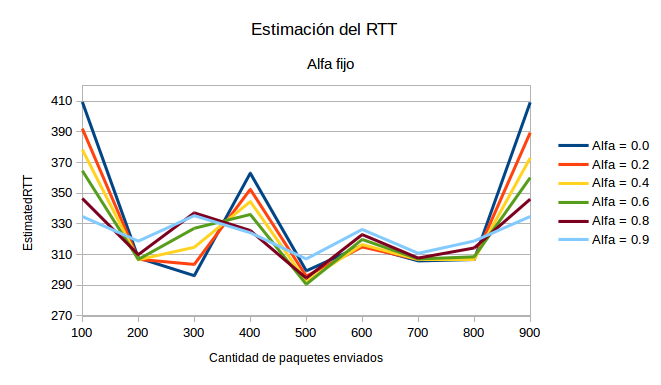
\includegraphics[width=0.8\textwidth]{imagenes/3ra_parte/ping_varios_alfa_fijo_variando_n_alemania.png}}

En el caso de la Universidad de Moscú, en general los valores fueron mas cercanos entre sí a pesar de incrementar la cantidad de paquetes a analizar. Pero al llegar a valores cercanos a los 900 paquetes, la estimación vuelve a crecer mas lentamente para valores de alfa mayores en comparación con los valores inferiores. 

Comenzamos a considerar que esto puede ser una tendencia real y que efectivamente las estimaciones con un alfa mas grande se normalizan mejor frente a un valor promedio en contraposición a las estimaciones que utilizan coeficientes alfa mucho menores, donde las mismas sufren de variaciones mucho mayores.

\centerline{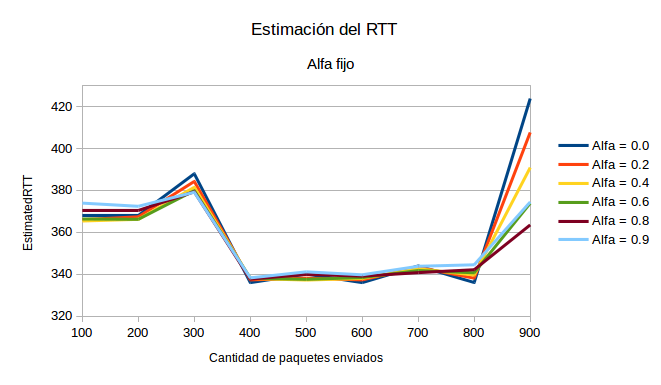
\includegraphics[width=0.8\textwidth]{imagenes/3ra_parte/ping_varios_alfa_fijo_variando_n_rusia.png}}

La Universidad de Tokio no es la excepción y vemos como ocurre nuevamente la misma situación. Sin importar la cantidad de paquetes ICMP enviados al host de la institución, las estimaciones hechas con valores de alfa superiores, son mucho mas estables entre sí con respecto a las estimaciones restantes.

\centerline{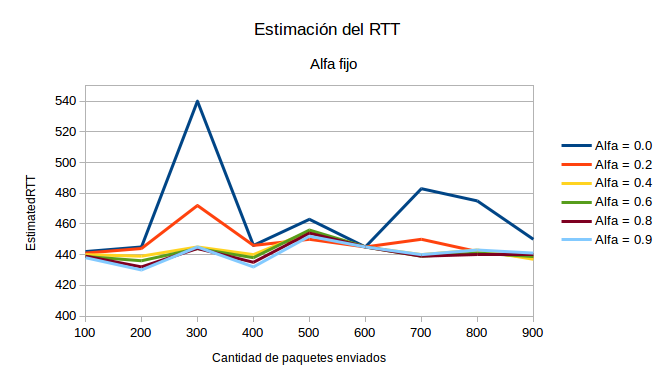
\includegraphics[width=0.8\textwidth]{imagenes/3ra_parte/ping_varios_alfa_fijo_variando_n_japon2.png}}

Finalmente, la Universidad de Boston refleja la situación que venimos remarcando de una manera aún mas clara. Se observa claramente como las estimaciones que utilizan el valor de alfa mas grande, son las mas estables a lo largo de los diferentes experimentos con las diversas cantidades de paquetes.

\centerline{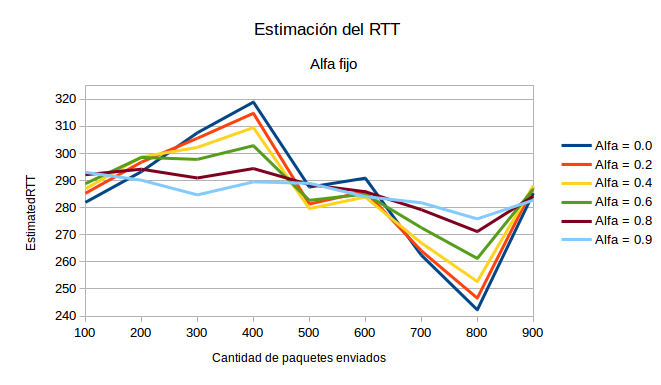
\includegraphics[width=0.8\textwidth]{imagenes/3ra_parte/ping_varios_alfa_fijo_variando_n_eeuu.png}}

\subsection{Estimación de RTT con cantidad fija de paquetes}

Ahora realizaremos una nueva serie de experimentos con las mismas muestras de RTT's obtenidas originalmente, pero esta vez fijaremos algunos subconjuntos con diferentes cantidades y veremos como van variando las estimaciones al incrementar el alfa para cada caso.

Para nuestra primer universidad, Humboldt de Berlín, observamos como en los tres casos al aumentar el coeficiente, todas las curvas tienden a un valor común, cercano a los 330. En aquellos casos donde las mediciones comenzaron por debajo de la estimación final, las estimaciones parciales fueron aumentando en tendencia a acercarse a dicho valor. En contrapartida, la curva que comenzó con mediciones superiores a la estimación final, terminó tendiendo a minimizar sus estimaciones parciales.

\centerline{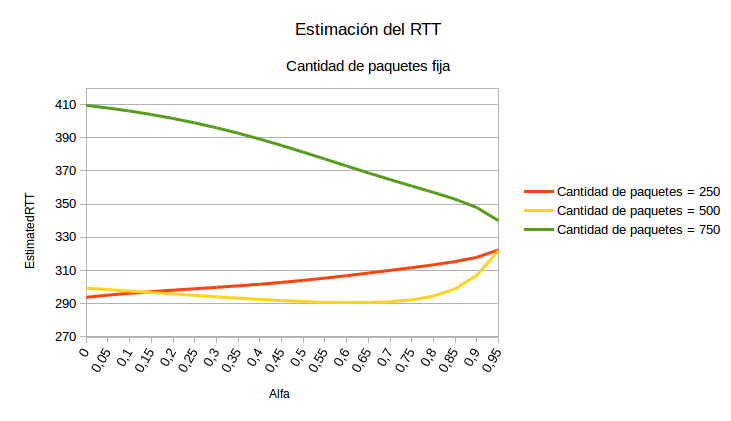
\includegraphics[width=0.8\textwidth]{imagenes/3ra_parte/ping_varios_n_fijo_variando_alfa_alemania.png}}

En el caso de la Universidad de Moscú, los valores se mantuvieron muy estables y cercanos entre sí, presentando una ligera aproximación de todas las curvas al final del experimento, al incrementar el valor de alfa.

\centerline{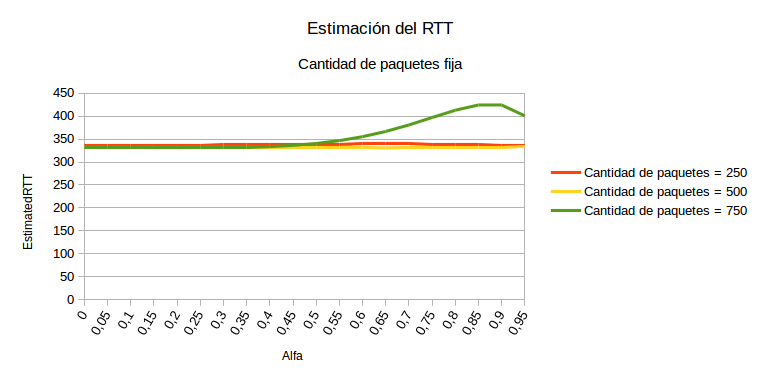
\includegraphics[width=0.8\textwidth]{imagenes/3ra_parte/ping_varios_n_fijo_variando_alfa_rusia.png}}

La gráfica de la Universidad de Tokio es un poco particular, mostrando crecimientos en todas las curvas (en mayor o menor medida) al aumentar el alfa del cálculo de estimaciones. Esto no quita que finalmente los valores tiendan a acercarse a un valor común, representado por el alcanzado en la curva con mayor cantidad de paquetes.

\centerline{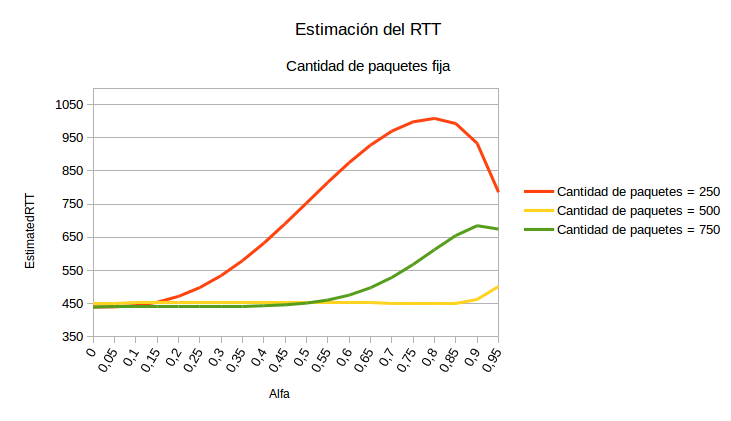
\includegraphics[width=0.8\textwidth]{imagenes/3ra_parte/ping_varios_n_fijo_variando_alfa_japon.png}}

El caso de la Universidad de Boston es el más explícito de todos, revelando como al aumentar por completo el alfa, las estimaciones convergen a un mismo valor, que resulta ser cercano al promedio de las estimaciones parciales.

\centerline{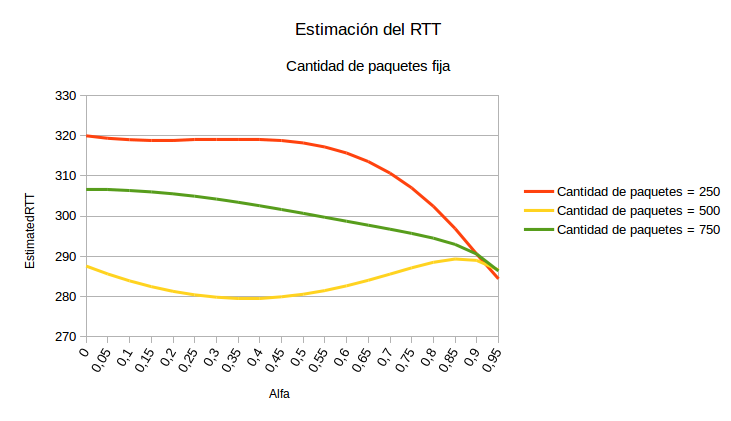
\includegraphics[width=0.8\textwidth]{imagenes/3ra_parte/ping_varios_n_fijo_variando_alfa_eeuu.png}}

\subsection{Estimaciones del RTT}

Teniendo los resultados correspondientes a cada universidad según ambos experimentos, consideramos las estimaciones con mayor valor de alfa (para aquellos con alfa fijo) y el valor promedio al que tienden las curvas (en el caso con cantidad fija de paquetes). La siguiente tabla condensa la información previamente descripta:

\begin{center}
 \begin{tabular}{|c||c|c|c|c|}
    \hline
    Universidad & Berlín & Moscú & Tokio & Boston \\ \hline \hline
    Estimación RTT con alfa fijo & 324,22 & 356,33 & 441,66 & 286,10 \\ \hline
    Estimación con cant. pings fijo & 328 & 354,66 & 655 & 286 \\ \hline
 \end{tabular}
\end{center}

\subsection{Estimación de la probabilidad de pérdida de paquetes}

Al enviar los ping originales a cada una de las universidades con las que estamos trabajando, no sólo habíamos calculado el tiempo insumido (los RTT's), sino que también habíamos contabilizado la cantidad de pings de los cuales no se obtuvo respuesta por parte de cada uno de los hosts. 

Para este experimento, nos dimos cuenta que la cantidad original de pings no era lo suficientemente amplia como para poder apreciar bien la pérdida de paquetes (con 1000 paquetes, hubo ocasiones donde no hubo ninguna pérdida). Por lo tanto incrementamos la cantidad de pings a enviar. Se pasó de mil a diez mil, y se volvió a ejecutar el script.

En base a los datos resultantes, estimaremos entonces cual es la probabilidad de perder un paquete en una conexión con los hosts de dichas instituciones. La fórmula utilizada es la siguiente:

\begin{equation}
EstimatedPacketLossProbability = 1 - \frac{\#Echo reply}{\#Echo request}
\end{equation}

En la siguiente tabla resumimos los datos obtenidos:

\begin{center}
 \begin{tabular}{|c||c|c|c|c|}
    \hline
    Universidad & Berlín & Moscú & Tokio & Boston \\ \hline \hline
    \#Echo request & 10000 & 10000 & 10000 & 10000 \\ \hline
    \#Echo reply & 9984 & \#\#\#\# & 9997 & 9953 \\ \hline
    EstimatedPacketLossProbability & 0,0016 & \#\#\#\# & 0,0003 & 0,0047 \\ \hline
 \end{tabular}
\end{center}

Cabe destacar, que en el caso de la Universidad de Moscú, a pesar de realizarse reiteradas pruebas con un importante número de paquetes, no se encontraron paquetes perdidos. 

\subsection{Contrastando las estimaciones con resultados previos}
En esta parte del trabajo práctico, se realizaron estimaciones sobre los valores de RTT posibles. A continuación quisieramos presentar, para recordar, los valores premedios de RTT obtenidos utilizando un traceroute desarrollado para las cuatro Universidades: 

\begin{center}
 \begin{tabular}{|c||c|c|c|c|}
    \hline
    Universidad & Berlín & Moscú & Tokio & Boston \\ \hline \hline
    RTT traceroute & 308,98 & 329.81 & 441.56 & 304.30 \\ \hline
 \end{tabular}
\end{center}

Estos tiempos entran dentro de los márgenes de valores que se observan en los gráficos del RTT estimado. Cuando los valores se estabilizaron para cierto $\alpha$ y $n$, los mismo no presentan una diferencia importante con los obtenidos en la primera sección del presente trabajo práctico. 

%\subsection{Simulación del throughput}
%
%Resolver la ecuación de Mantis para cada universidad?
%
%Datos a tener en cuenta:
%
%* MSS: es el Maximum Segment Size. 
%Aparentemente MSS $=$ MTU $-$ TCP/IP headers.
%
%Ejemplo encontrado en: alouche.net/blog/2009/09/16/mathis-equation-and-tcp-performance/
%MSS = MTU - TCP/IP headers - for example 1460 with an MTU of 1500 (20b IP and 20b TCP headers)
%
%* MTU: es el Maximum Transfer Unit.
%\url{https://es.wikipedia.org/wiki/Unidad_máxima_de_transferencia}
%
%\begin{equation}
%BandWidth = \frac{data\ per\ cycle}{time\ per\ cycle} = \frac{MSS * \sqrt{\frac{3}{2}}}{EstimatedRTT * %sqrt{EstimatedPacketLossProbability}}
%\end{equation}

\newpage
\section{Conclusión}

A lo largo del trabajo práctico, se fueron realizando diversos experimentos para poder comprender el comportamiento de la red mundia, por donde se transmiten millones de paquetes todo el tiempo. Se pudo observar que un mensaje enviado desde un host a otro, realiza un recorrido inmenso, saltando por diversos host intermedios. Cada host intermedio, presenta un comportamiento completamente diferente y hace al aumento del tiempo en el que llegará un paquete a destino. 

En este trabajo práctico se observaron muchos router que no tenían habilitado un sistema de respuesta, por lo que presentó dificultades al momento de realizar los análisis necesarios. Estos hops intermedios fueron ignorados completamente, para tratar de afectar lo menos posible al RTT promedio. Además, se pudo notar, que dependiendo del día o del momento, en el cual se realizan las mediciones, el tiempo total obtenido es notablemente diferente. 

Creemos que se podrían haber realizado análisis más profundos, quizás tomando medicientes cada diez minutos durante todo un día, pero probablemente los RTT para cada hop intermedio no se diferenciarían mucho de los actuales. 
\end{document}
